%%%%%%%%%%%%%%%%%%%%%%%%%%%%%%%%%%%%%%%%%%%%%%%%%%%%%%
%   TeXstudio as your IDE
%%  برای compile در TeXstudio تنها کافی است منوی Options->Configure TeXstudio را زده و در پنجره Configure TeXstudio در بخش Build گزینه Default Compiler را به XeLaTeX تغییر دهید. سند شما به راحتی compile خواهد شد.
%   F1 & F5 : Build & view
%   F6      : Compile
%   F7      : View
%   --------------
%%%%%%%%%%%%%%%%%%%%%%%%%%%%%%%%%%%%%%%%%%%%%%%%%%%%%%
%%% !TEX TS-program = XeLaTeX
\documentclass[oneside,msc,12pt]{AUTthesis}
%% توجه شود برای نسخه نهایی پایان‌نامه حتماً hyperref را غیرفعال کنید.

% در این فایل، دستورها و تنظیمات مورد نیاز، آورده شده است.
%-------------------------------------------------------------------------------------------------------------------
% در ورژن جدید زی‌پرشین برای تایپ متن‌های ریاضی، این سه بسته، حتماً باید فراخوانی شود.
\usepackage{amsthm,amssymb,amsmath,amsfonts}
% بسته‌ای برای تنطیم حاشیه‌های بالا، پایین، چپ و راست صفحه
\usepackage[top=30mm, bottom=30mm, left=25mm, right=30mm]{geometry}
% بسته‌‌ای برای ظاهر شدن شکل‌ها و تصاویر متن
\usepackage{graphicx}
\usepackage{color}
%بسته‌ای برای تنظیم فاصله عمودی خط‌های متن
\usepackage{setspace}
\usepackage{titletoc}
\usepackage{tocloft}
%با فعال کردن بسته زیر فوت‌نوت‌ها در هر صفحه ریست می‌شوند. حالت پیش‌فرض آن ریست شدن در هر فصل می‌باشد.
%\usepackage[perpage]{footmisc}
\usepackage{enumitem}
\usepackage{multirow,adjustbox}
%\usepackage{titlesec}
% بسته‌ و دستوراتی برای ایجاد لینک‌های رنگی با امکان جهش
\usepackage[pagebackref=false,colorlinks,linkcolor=blue,citecolor=red]{hyperref}
\usepackage[nameinlink]{cleveref}%capitalize,,noabbrev
 \AtBeginDocument{%
    \crefname{equation}{برابری}{equations}%
    \crefname{chapter}{فصل}{chapters}%
    \crefname{section}{بخش}{sections}%
    \crefname{appendix}{پیوست}{appendices}%
    \crefname{enumi}{مورد}{items}%
    \crefname{footnote}{زیرنویس}{footnotes}%
    \crefname{figure}{شکل}{figures}%
    \crefname{table}{جدول}{tables}%
    \crefname{theorem}{قضیه}{theorems}%
    \crefname{lemma}{لم}{lemmas}%
    \crefname{corollary}{نتیجه}{corollaries}%
    \crefname{proposition}{گزاره}{propositions}%
    \crefname{definition}{تعریف}{definitions}%
    \crefname{result}{نتیجه}{results}%
    \crefname{example}{مثال}{examples}%
    \crefname{remark}{نکته}{remarks}%
    \crefname{note}{یادداشت}{notes}%
    \crefname{asum}{فرض}{Assumption}
    % دستوری برای تغییر نام کلمه «کتاب‌نامه» به «منابع و مراجع«
    \renewcommand{\bibname}{منابع و مراجع}
    
    \renewcommand{\labelitemi}{$\bullet$}
    % دستوری برای تعیین علامت سطح دوم itemize
    \renewcommand{\labelitemii}{$\circ$}
    % دستوری برای تعیین علامت سطح سوم itemize
    \renewcommand{\labelitemiii}{$-$}
    % برای سطح چهارم
    \renewcommand{\labelitemiv}{$*$}
    % دستوری برای تغییر نام کلمه «اثبات» به «برهان»
    \renewcommand\proofname{\textbf{برهان}}
    \renewcommand{\listfigurename}{فهرست اشکال}
    \renewcommand{\listtablename}{فهرست جداول}
}

\usepackage{subcaption}
% چنانچه قصد پرینت گرفتن نوشته خود را دارید، خط بالا را غیرفعال و  از دستور زیر استفاده کنید چون در صورت استفاده از دستور زیر‌‌، 
% لینک‌ها به رنگ سیاه ظاهر خواهند شد که برای پرینت گرفتن، مناسب‌تر است
%\usepackage[pagebackref=false]{hyperref}
% بسته‌ لازم برای تنظیم سربرگ‌ها
\usepackage{fancyhdr}
% بسته‌ای برای ظاهر شدن «مراجع»  در فهرست مطالب
\usepackage[nottoc]{tocbibind}
% دستورات مربوط به ایجاد نمایه
\usepackage{makeidx,multicol}
\setlength{\columnsep}{1.5cm}

%%%%%%%%%%%%%%%%%%%%%%%%%%
\usepackage{verbatim}
\makeindex
\usepackage{sectsty}
% فراخوانی بسته زی‌پرشین و تعریف قلم فارسی و انگلیسی
\usepackage{xepersian}%[extrafootnotefeatures]
\SepMark{-}
%حتماً از تک لایو 2014 استفاده کنید.
\settextfont[Scale=1.2,Path=Fonts/,BoldFont=B Nazanin Bold.ttf]{B Nazanin.ttf}
\setlatintextfont[Path=Fonts/,BoldFont=timesbd]{times}

%%%%%%%%%%%%%%%%%%%%%%%%%%
% چنانچه می‌خواهید اعداد در فرمول‌ها، انگلیسی باشد، خط زیر را غیرفعال کنید.
%
\setdigitfont[Scale=1.1,Path=Fonts/,BoldFont=Yas Bd.ttf]{Yas.ttf}%%Yas
%%%%%%%%%%%%%%%%%%%%%%%%%%
% تعریف قلم‌های فارسی اضافی برای استفاده در بعضی از قسمت‌های متن
\defpersianfont\nastaliq[Scale=2,Path=Fonts/]{IranNastaliq.ttf}
\defpersianfont\chapternumber[Scale=3,Path=Fonts/,BoldFont=B Nazanin Bold.ttf]{B Nazanin.ttf}
%\chapterfont{\centering}%
%%%%%%%%%%%%%%%%%%%%%%%%%%





% Headings for every page of ToC, LoF and Lot
\setlength{\cftbeforetoctitleskip}{-1.2em}
\setlength{\cftbeforelottitleskip}{-1.2em}
\setlength{\cftbeforeloftitleskip}{-1.2em}
\setlength{\cftaftertoctitleskip}{-1em}
\setlength{\cftafterlottitleskip}{-1em}
\setlength{\cftafterloftitleskip}{-1em}
%%\makeatletter
%%%%\renewcommand{\l@chapter}{\@dottedtocline{1}{1em\bfseries}{1em}}
%%%%\renewcommand{\l@section}{\@dottedtocline{2}{2em}{2em}}
%%%%\renewcommand{\l@subsection}{\@dottedtocline{3}{3em}{3em}}
%%%%\renewcommand{\l@subsubsection}{\@dottedtocline{4}{4em}{4em}}
%%%%\makeatother


\newcommand\tocheading{\par عنوان\hfill صفحه \par}
\newcommand\lofheading{\hspace*{.5cm}\figurename\hfill صفحه \par}
\newcommand\lotheading{\hspace*{.5cm}\tablename\hfill صفحه \par}

\renewcommand{\cftchapleader}{\cftdotfill{\cftdotsep}}
\renewcommand{\cfttoctitlefont}{\hspace*{\fill}\LARGE\bfseries}%\Large
\renewcommand{\cftaftertoctitle}{\hspace*{\fill}}
\renewcommand{\cftlottitlefont}{\hspace*{\fill}\LARGE\bfseries}%\Large
\renewcommand{\cftafterlottitle}{\hspace*{\fill}}
\renewcommand{\cftloftitlefont}{\hspace*{\fill}\LARGE\bfseries}
\renewcommand{\cftafterloftitle}{\hspace*{\fill}}

%%%%%%%%%%%%%%%%%%%%%%%%%%
% تعریف و نحوه ظاهر شدن عنوان قضیه‌ها، تعریف‌ها، مثال‌ها و ...
%برای شماره گذاری سه تایی قضیه ها
\theoremstyle{definition}
\newtheorem{definition}{تعریف}[section]
\newtheorem{remark}[definition]{نکته}
\newtheorem{note}[definition]{یادداشت}
\newtheorem{example}[definition]{نمونه}
\newtheorem{question}[definition]{سوال}
\newtheorem{remember}[definition]{یاداوری}
\theoremstyle{theorem}
\newtheorem{theorem}[definition]{قضیه}
\newtheorem{lemma}[definition]{لم}
\newtheorem{proposition}[definition]{گزاره}
\newtheorem{corollary}[definition]{نتیجه}
\newtheorem{asum}[definition]{فرض}
%%%%%%%%%%%%%%%%%%%%%%%%
%%%%%%%%%%%%%%%%%%%
%%% برای شماره گذاری چهارتایی قضیه ها و ...
%%\newtheorem{definition1}[subsubsection]{تعریف}
%%\newtheorem{theorem1}[subsubsection]{قضیه}
%%\newtheorem{lemma1}[subsubsection]{لم}
%%\newtheorem{proposition1}[subsubsection]{گزاره}
%%\newtheorem{corollary1}[subsubsection]{نتیجه}
%%\newtheorem{remark1}[subsubsection]{نکته}
%%\newtheorem{example1}[subsubsection]{مثال}
%%\newtheorem{question1}[subsubsection]{سوال}

%%%%%%%%%%%%%%%%%%%%%%%%%%%%

% دستورهایی برای سفارشی کردن صفحات اول فصل‌ها
\makeatletter
\newcommand\mycustomraggedright{%
 \if@RTL\raggedleft%
 \else\raggedright%
 \fi}
\def\@makechapterhead#1{%
\thispagestyle{style1}
\vspace*{20\p@}%
{\parindent \z@ \mycustomraggedright
\ifnum \c@secnumdepth >\m@ne
\if@mainmatter

\bfseries{\Huge \@chapapp}\small\space {\chapternumber\thechapter}
\par\nobreak
\vskip 0\p@
\fi
\fi
\interlinepenalty\@M 
\Huge \bfseries #1\par\nobreak
\vskip 120\p@

}

%\thispagestyle{empty}
\newpage}
\bidi@patchcmd{\@makechapterhead}{\thechapter}{\tartibi{chapter}}{}{}
\bidi@patchcmd{\chaptermark}{\thechapter}{\tartibi{chapter}}{}{}
\makeatother

\pagestyle{fancy}
\renewcommand{\chaptermark}[1]{\markboth{\chaptername~\tartibi{chapter}: #1}{}}

\fancypagestyle{style1}{
\fancyhf{} 
\fancyfoot[c]{\thepage}
\fancyhead[R]{\leftmark}%
\renewcommand{\headrulewidth}{1.2pt}
}


\fancypagestyle{style2}{
\fancyhf{}
\fancyhead[R]{چکیده}
\fancyfoot[C]{\thepage{}}
\renewcommand{\headrulewidth}{1.2pt}
}

\fancypagestyle{style3}{%
  \fancyhf{}%
  \fancyhead[R]{فهرست نمادها}
  \fancyfoot[C]{\thepage}%
  \renewcommand{\headrulewidth}{1.2pt}%
}

\fancypagestyle{style4}{%
  \fancyhf{}%
  \fancyhead[R]{فهرست جداول}
  \fancyfoot[C]{\thepage}%
  \renewcommand{\headrulewidth}{1.2pt}%
}

\fancypagestyle{style5}{%
  \fancyhf{}%
  \fancyhead[R]{فهرست اشکال}
  \fancyfoot[C]{\thepage}%
  \renewcommand{\headrulewidth}{1.2pt}%
}

\fancypagestyle{style6}{%
  \fancyhf{}%
  \fancyhead[R]{فهرست مطالب}
  \fancyfoot[C]{\thepage}%
  \renewcommand{\headrulewidth}{1.2pt}%
}

\fancypagestyle{style7}{%
  \fancyhf{}%
  \fancyhead[R]{نمایه}
  \fancyfoot[C]{\thepage}%
  \renewcommand{\headrulewidth}{1.2pt}%
}

\fancypagestyle{style8}{%
  \fancyhf{}%
  \fancyhead[R]{منابع و مراجع}
  \fancyfoot[C]{\thepage}%
  \renewcommand{\headrulewidth}{1.2pt}%
}
\fancypagestyle{style9}{%
  \fancyhf{}%
  \fancyhead[R]{واژه‌نامه‌ی فارسی به انگلیسی}
  \fancyfoot[C]{\thepage}%
  \renewcommand{\headrulewidth}{1.2pt}%
}
%


%دستور حذف نام لیست تصاویر و لیست جداول از فهرست مطالب
\newcommand*{\BeginNoToc}{%
  \addtocontents{toc}{%
    \edef\protect\SavedTocDepth{\protect\the\protect\value{tocdepth}}%
  }%
  \addtocontents{toc}{%
    \protect\setcounter{tocdepth}{-10}%
  }%
}
\newcommand*{\EndNoToc}{%
  \addtocontents{toc}{%
    \protect\setcounter{tocdepth}{\protect\SavedTocDepth}%
  }%
}
\newcounter{savepage}

%\renewcommand\cftsecleader{\cftdotfill{\cftdotsep}}
%%%%%%%%%%%%%%%%%%%%%%%%%%%%%
%%%%%%%%%%%%%%%%%%%%%%%%%%%%

\begin{document}
\baselineskip=.75cm
\linespread{1.75}
%% -!TEX root = AUTthesis.tex
% در این فایل، عنوان پایان‌نامه، مشخصات خود، متن تقدیمی‌، ستایش، سپاس‌گزاری و چکیده پایان‌نامه را به فارسی، وارد کنید.
% توجه داشته باشید که جدول حاوی مشخصات پروژه/پایان‌نامه/رساله و همچنین، مشخصات داخل آن، به طور خودکار، درج می‌شود.
%%%%%%%%%%%%%%%%%%%%%%%%%%%%%%%%%%%%
% دانشکده، آموزشکده و یا پژوهشکده  خود را وارد کنید
\faculty{دانشکده مهندسی کامپیوتر}
% گرایش و گروه آموزشی خود را وارد کنید
\department{}
% عنوان پایان‌نامه را وارد کنید
\fatitle{تقسیم‌بندی معنایی برای ماشین‌های خودران با استفاده از یادگیری عمیق
\\[.75 cm]
}
% نام استاد(ان) راهنما را وارد کنید
\firstsupervisor{دکتر احسان ناظرفرد}
%\secondsupervisor{استاد راهنمای دوم}
% نام استاد(دان) مشاور را وارد کنید. چنانچه استاد مشاور ندارید، دستور پایین را غیرفعال کنید.
%\firstadvisor{استاد مشاور اول}
%\secondadvisor{استاد مشاور دوم}
% نام نویسنده و نام خانوادگیرا وارد کنید
\name{کیوان}

\surname{ ایپچی حق }
%%%%%%%%%%%%%%%%%%%%%%%%%%%%%%%%%%
\thesisdate{فروردین ۱۴۰۳}

% چکیده پایان‌نامه را وارد کنید
\fa-abstract{
خودروهای خودران
\LTRfootnote{Self-driving cars}
به منظور اتخاذ تصمیمات آگاهانه و مسیریابی ایمن در محیط‌های مختلف، نیازمند درک دقیقی از اشیاء اطراف خود هستند. تقسیم‌بندی معنایی
\LTRfootnote{Semantic segmentation}
از ابتدایی‌ترین مراحل در فرایند تجزیه و تحلیل تصاویر و استخراج اطلاعات مفید آن به منظور تصمیم‌گیری در اینگونه سیستم‌ها است که نقش حیاتی در تشخیص اشیاء محیط دارد و این امکان را بوجود می‌آورد تا به طور دقیق اشیاء مختلف از جمله جاده‌ها، عابران پیاده، خودروهای دیگر و موانع شناسایی شوند. روش‌های یادگیری عمیق
\LTRfootnote{Deep learning}
بهبود قابل توجهی در تقسیم‌بندی معنایی تصاویر به وجود آورده‌اند، به گونه‌ای که از عملکرد برتری نسبت به روش‌های سنتی برخوردار هستند. این پروژه به بررسی پیشرفت‌های اخیر در زمینه تقسیم‌بندی معنایی تصاویر برای خودروهای خودران با استفاده از روش‌های یادگیری عمیق می‌پردازد. ما معماری‌های مختلف یادگیری عمیق را در مسئله تقسیم‌بندی معنایی سریع
\LTRfootnote{Fast semantic segmentation}
مورد مطالعه قرار داده، معماری‌های مختلف را مقایسه نموده و نقاط قوت و ضعف آنها را برای مسئله خاص خودروهای خودران بررسی می‌کنیم. علاوه بر این، مجموعه‌داده‌های مورد استفاده برای آموزش و ارزیابی مدل‌های تقسیم‌بندی معنایی در این حوزه مورد بررسی قرار گرفته و از آنها برای ارزیابی مدل‌های یادگیری عمیق مختلف استفاده می‌شود. در پایان، جمع‌بندی بر روی مدل‌های مورد بررسی قرار گرفته خواهیم داشت و پیشنهاداتی برای پژوهش‌های آینده در جهت بهبود پایداری، کارایی و قابلیت عمومی سیستم‌های تقسیم‌بندی معنایی در لحظه مبتنی بر یادگیری عمیق برای خودروهای خودران ارائه می‌شود.
}

% کلمات کلیدی پایان‌نامه را وارد کنید
\keywords{هوش مصنوعی، خودرو‌های خودران، یادگیری عمیق، تقسیم بندی معنایی، تقسیم‌بندی معنایی سریع تصاویر}



\AUTtitle
%%%%%%%%%%%%%%%%%%%%%%%%%%%%%%%%%%
\vspace*{7cm}
\thispagestyle{empty}
\begin{center}

\includegraphics[height=5cm,width=12cm]{Images/besm.jpg}
\end{center}
% تاییدیه دفاع
\newpage
\thispagestyle{empty}
\begin{picture}(50,50)
  \put(17,0){
\includegraphics[scale=1.1]{fa-logo.png}}
  \put(4.5,-13){\footnotesize{دانشگاه صنعتی امیرکبیر}}
  \put(10.5,-27){\footnotesize{(پلی‌تکنیک تهران)}}
  \put(170,30){\bf{به نام خدا}}
  \put(140,-5){\Large\bf{تعهدنامه اصالت اثر}}
  \put(310,0){تاریخ: \datethesis}
\end{picture}

\vspace*{2.5cm}

اينجانب {\bf{\fname\lname}} متعهد می‌شوم که مطالب مندرج در این پایان‌نامه حاصل کار پژوهشی اینجانب تحت نظارت و راهنمایی اساتید دانشگاه صنعتی امیرکبیر بوده و به دستاوردهای دیگران که در این پژوهش از آنها استفاده شده است مطابق مقررات و روال متعارف ارجاع و در فهرست منابع و مآخذ ذکر گردیده است. این پایان‌نامه قبلاً برای احراز هیچ مدرک هم‌سطح یا بالاتر ارائه نگردیده است.

در صورت اثبات تخلف در هر زمان، مدرک تحصیلی صادر شده توسط دانشگاه از درجه اعتبار ساقط بوده و دانشگاه حق پیگیری قانونی خواهد داشت.


کلیه نتایج و حقوق حاصل از این پایان‌نامه متعلق به دانشگاه صنعتی امیرکبیر می‌باشد. هرگونه استفاده از نتایج علمی و عملی، واگذاری اطلاعات به دیگران یا چاپ و تکثیر، نسخه‌برداری، ترجمه و اقتباس از این پایان نامه بدون موافقت کتبی دانشگاه صنعتی امیرکبیر ممنوع است. 
نقل مطالب با ذکر مآخذ بلامانع است.\\
\vspace{2.5cm}


{\centerline {\bf{\fname\lname}}}
\vspace*{.2cm}
{\centerline{امضا}}
%%%%%%%%%%%%%%%%%%%%%%%%%%%%%%%%%
% نیایش خود را در فایل زیر بنویسید.
\begin{acknowledgementpage}

\vspace{1.5cm}

{\nastaliq
{
	تقدیم به
	
 آنان که الفبای انسانیت و چگونه زیستن را به من آموختند...
}}\end{acknowledgementpage}
\newpage
% سپاسگزاری را در فایل زیر بنویسید.
%%%%%%%%%%%%%%%%%%%%%%%%%%%%%%%%%%%%
\newpage\thispagestyle{empty}
% سپاس‌گزاری
{\nastaliq
سپاس‌گزاری
}
\\[2cm]

 بدین وسیله از زحمات و تلاش بی‌دریغ استاد محترم جناب دکتر احسان ناظرفرد و خانواده عزیزم صمیمانه سپاسگزاری می نمایم و همچنین از سایر همکاران و دوستانی که هر کدام به نحوی در تهیه این مجموعه با این جانب همکاری داشته اند تشکر نموده و موفقیت همه آنها را از خداوند متعال خواهانم.














% با استفاده از دستور زیر، امضای شما، به طور خودکار، درج می‌شود.
\signature








%%%%%%%%%%%%%%%%%%%%%%%%%%%%%%%%%%%%%%%%%
%%%%%%%%%%%%%%%%%%%%%%%%%%%%%%%%%کدهای زیر را تغییر ندهید.
\newpage\clearpage

\pagestyle{style2}

\vspace*{-1cm}
\section*{\centering چکیده}
%\addcontentsline{toc}{chapter}{چکیده}
\vspace*{.5cm}
\ffa-abstract
\vspace*{2cm}


{\noindent\large\textbf{واژه‌های کلیدی:}}\par
\vspace*{.5cm}
\fkeywords
% دستور زیر برای شماره گذاری صفحات قبل از فصل اول با حروف ابجد است.
\pagenumbering{alph}
%-----------------------------------------------------------------------------
% فایل زیر دستورات مربوط به نمایش صفحات فهرست مطالب- فهرست اشکال و جداول است.
%{\pagestyle{style2}
%\tableofcontents}\newpage
%
%\listoffigures
\cleardoublepage
\pagestyle{style6}
\tableofcontents
\pagestyle{style6}
\cleardoublepage
%اگر لیست تصاویر و لیست جداول ندارید ، کدهای زیر را با گذاشتن % در ابتدای آنها، غیرفعال کنید.
\BeginNoToc
%============
\addtocontents{lof}{\lofheading}% add heading to the first page in LoF
\pagestyle{style5}
\listoffigures
\thispagestyle{style5}
\cleardoublepage
%============
\addtocontents{lot}{\lotheading}% add heading to the first page in LoT
\thispagestyle{style4}
\listoftables
\thispagestyle{style4}
%============
%\cleardoublepage
%
\cleardoublepage
\setcounter{savepage}{\arabic{page}}
\mainmatter
\addtocontents{toc}{\tocheading}% add heading to the first page in ToC, after frontmatter entries
\EndNoToc
% در صورت تمایل می‌توانید با فعال کردن دستور بالا، لیست تصاویر را به  پایان‌نامه خود اضافه کنید.
%-------------------------------------------------------------------------symbols(فهرست نمادها)
% وجود لیست نمادها الزامیست.(لطفاً نمادهای خود را جایگذین نمادهای پیش‌فرض کنید.)
%%%%%%%%%%%%%

{\centering\LARGE\textbf{فهرست نمادها}\par}%

\pagenumbering{alph}
\setcounter{page}{\thesavepage}
%\setcounter{page}{6}
\vspace*{1cm}

\pagestyle{style3}
%\thispagestyle{empty}
%\addcontentsline{toc}{chapter}{فهرست نمادها}
\symb{\text{ نماد}}{مفهوم}
\\
%مقادیر بالا را تغییر ندهید
%%%%%%%%%%%%%%%%%%%%%%%%%%%%%%%%%%%%%%%%%%%%%%%%%%%%%%%%%
\symb{\mathbb{R}^n}{
فضای اقلیدسی با بعد $n$
}
\symb{\mathbb{S}^n}{
کره یکه $n$ بعدی
}
\symb{M^m}{
خمینه $m$-بعدی $M$
}
\symb{\mathfrak{X}(M)}{
جبر میدان‌های  برداری هموار روی $M$
}
\symb{\mathfrak{X}^1(M)}{
مجموعه میدان‌های برداری هموار یکه روی $(M,g)$ 
}
\symb{\Omega^p(M)}{
مجموعه $p$-فرمی‌های روی خمینه $M$
}
\symb{Q}{
اپراتور ریچی
}
\symb{\mathcal{R}}{
تانسور انحنای ریمان
}
\symb{ric}{
تانسور ریچی
}
\symb{L}{
مشتق لی
}
\symb{\Phi}{
2-فرم اساسی خمینه تماسی
}
\symb{\nabla}{
التصاق لوی-چویتای
}
\symb{\Delta}{
لاپلاسین ناهموار
}
\symb{\nabla^*}{
عملگر خودالحاق صوری القا شده از التصاق لوی-چویتای
}
\symb{g_s}{
متر ساساکی
}
\symb{\nabla}{
التصاق لوی-چویتای وابسته به متر ساساکی
}
\symb{\Delta}{
عملگر لاپلاس-بلترامی روی $p$-فرم‌ها
}

%%%%%%%%%%%%%%%%%%%%%%%%%%%%%%%%%%%%%%%

\thispagestyle{style3}
\newpage
%\pagestyle{style1}
%%%%%%%%%%%%%%%%%%%%%%%%%%%%%%%%%%%%


\pagenumbering{arabic}
\pagestyle{style1}
%--------------------------------------------------------------------------chapters(فصل ها)
\chapter{مقدمه}

\section{شرح مسأله}
در دهه اخیر، پیشرفت‌های چشمگیری در زمینه هوش مصنوعی و یادگیری عمیق، به ویژه در حوزه پردازش تصویر و استفاده از آنها برای بهبود عملکرد تصمیم‌گیری در خودروهای خودران، انقلابی در روند توسعه و بهینه‌سازی فناوری در این زمینه ایجاد کرده است. شبکه‌های عصبی عمیق
\LTRfootnote{Deep neural networks}
به دلیل قابلیت‌هایی که از طریق شبکه‌های عصبی کانولوشنی
\LTRfootnote{convolutional neural networks}
\cite{o2015introduction}
فراهم می‌آید، امکاناتی را برای خودروها فراهم می‌کند که پیش از این غیرقابل تصور بوده است.

با این وجود، یکی از چالش‌های بزرگ در مسیر توسعه خودروهای خودران، توانایی فهم و تفسیر دقیق محیط اطراف و اشیاء موجود در تصویر است. برای حل این چالش معمولاً از روش‌های متنوعی استفاده می‌شود که یکی از روش‌های مهم در این زمینه، تقسیم بندی معنایی نامیده می‌شود. در این روش، تمامی سلول‌‌های
\LTRfootnote{Pixel}
تصویری موجود به دسته‌هایی از پیش تعیین شده تخصیص داده می‌شوند. خودرو باید توانایی آن را داشته باشد تا اطلاعات دریافتی از محیط را با سرعت در لحظه
\LTRfootnote{Real-time}
به دسته‌های مختلف مانند خیابان، پیاده‌رو، خودروها، چراغ راهنما و غیره تقسیم بندی کرده و به هر دسته یک رنگ مخصوص که اسطلاحا به آن رنگبندی تقسیم‌بندی
\LTRfootnote{Segmentation color}
گفته می‌شود اختصاص دهد.

بدون شک، تقسیم‌بندی معنایی محیط برای خودروهای خودران امری بسیار اساسی و حیاتی است. اطلاعات دقیق و صحیح در مورد محیط اطراف، به سیستم‌های خودران امکان می‌دهد تا تصمیمات صحیح و ایمن را در مسیر حرکت خود اتخاذ کنند. این اطلاعات، پایه‌ای برای عملکرد امن و کارآمد این خودروهای خودران است. در عین اهمیت داشتن دقت بالا در انجام این امر، پردازش در لحظه نیز حائز اهمیت است. زیرا تنها داشتن دقت بالا بدون توانایی پردازش سریع و به موقع، در مسائلی که نیاز به پردازش آنی دارند ناکارآمد خواهد بود. به عبارتی دیگر، دقت بالا و سرعت پردازش به‌طور همزمان، می‌توانند به عنوان دو عامل اساسی و مکمل، عملکرد بهینه سیستم خودران را فراهم کنند.

\section{اهداف پروژه}
ادر بخش ابتدایی از پروژه، به توضیح مقدمه‌ای بر چگونگی انجام تقسیم‌بندی معنایی تصاویر پرداخته و سپس به بررسی روش‌های تقسیم‌بندی معنایی بااستفاده از یادگیری عمیق که برای استفاده در حوزه تصویربرداری پزشکی طراحی شده‌اند
\LTRfootnote{Medical Imaging}
می‌پردازیم. تمرکز ما در این بخش بررسی مدل‌هایی است که از دقت بالایی برخوردار هستند و سرعت عمل به عنوان یک مشخصه ثانویه مطرح نمی‌شود، زیرا هدف این مدل‌ها در صنعت پزشکی، تشخیص درست و دقیق اجزای موجود در تصویر است که سرعت حائز اهمیت چندانی نیست.
در ادامه، به بررسی روش‌های یادگیری عمیق برای تقسیم‌بندی معنایی در حوزه خودروهای خودران با تمرکز بر پردازش در لحظه پرداخته و هدف ما دقت بالا و سرعت عمل بهینه متناسب با این مسئله است. با توجه به نیازهای خاص این حوزه، ما به دنبال راهکارها و معماری‌هایی هستیم که بهبود دقت و سرعت عمل سیستم‌های خودران را به هدف داشته و در نتیجه، ایمنی و کارایی این سیستم‌ها را بهبود بخشند.
در پایان، به جمع‌بندی و نتیجه‌گیری مطالب بدست آمده در این پروژه پرداخته و مروری بر سیر انجام پروژه و معماری‌های مطرح شده خواهیم داشت و سپس پیشنهاداتی برای کار‌های آینده که می‌تواند به بهبود وضعیت فعلی کمک کند، مطرح می‌کنیم.

\section{ساختار گزارش}
در فصل ابتدایی این گزارش، مقدمه‌ای بر روی مسأله مطرح شده در این پروژه و شرح کلی از اهداف و محتوای گزارش ارائه شد. در فصل دوم، به طور مفصل به مفاهیم مرتبط و چگونگی پیاده‌سازی این مسأله پرداخته و سپس به بررسی معماری رمزگذار-رمزگشا و مدل‌هایی که از این معماری استفاده می‌کنند پرداخته خواهد شد. در فصل سوم، به مدل‌های طراحی شده برای مساله خاص تقسیم‌بندی معنایی در خودروهای خودران اشاره شده و سپس مدل‌های پیشنهادی این پژوهش انتخاب و به طور مفصل توضیح داده خواهد شد. در فصل چهارم، آزمایش‌ها، نتایج و ارزیابی‌های انجام شده بر روی کیفیت و کارایی مدل‌ها مورد بحث و بررسی قرار خواهند گرفت. در فصل پنجم، به عنوان فصل پایانی، جمع‌بندی نکات گزارش و پیشنهاد‌هایی برای کارهای آینده به منظور بهبود عملکرد و کارایی در این حوزه خواهد شد.
\chapter{مرور کار‌های پیشین}

\section{مقدمه‌ای تقسیم‌بندی معنایی}

در مسأله تقسیم‌بندی معنایی، مدل یک نقشه تقسیم‌بندی شده
\LTRfootnote{Segmentation map}
از شناسه‌ها
\LTRfootnote{Segmentation id}
را تولید می‌کند که هر سلول تصویر به یک شناسه خاص مرتبط با دسته‌بندی هر شیء اختصاص می‌یابد. این نقشه تقسیم‌بندی شده در واقع یک تصویر خاکستری دو بعدی
\LTRfootnote{Grayscale image}
است، زیرا صرفا شامل شناسه ها که خود اعداد کوچک بوده است که باعث می‌شوند تصویر تیره و با تنها یک کانال رنگی تولید شود که در آن هر مقدار سلول متناظر با شناسه دسته شیء مورد نظر است که نمایانگر دسته آن شیء است. به عنوان مثال، در یک نقشه تقسیم‌بندی شده، مقادیر پیکسل ۱ ممکن است نمایانگر زمینه باشد، مقادیر ۲ ممکن است نمایانگر یک عابر پیاده و مقادیر ۳ ممکن است نمایانگر یک خودرو باشد و غیره.

تمایز بین اشیاء موجود در یک تصویر خاکستری برای چشم انسان کار دشواری است. به همین دلیل، برای تبدیل این نقشه تقسیم‌بندی خاکستری به یک تصویر تقسیم‌بندی شده رنگارنگ
\LTRfootnote{Segmentation image}
که به صورت بصری شیء‌های تقسیم‌بندی شده را نشان می‌دهد، از یک تبدیل بین رنگ‌ها به شناسه‌ها و برعکس آن استفاده می‌شود. این تبدیل شامل اختصاص رنگ‌های متمایز به هر دسته (شناسه اشیاء) است. رویکرد رایج‌تر، استفاده از یک پالت رنگ
\LTRfootnote{Color palette}
پیش‌تعیین شده است که هر کلاس با یک کد رنگی
\LTRfootnote{RGBA}
منحصر به فرد مرتبط است.

از این تبدیل برای تغییر تصاویر رنگارنگ به خاکستری قبل از دادن آنها به مدل و برعکس آن بر روی خروجی مدل استفاده می‌شود. به طوری که تصاویر رنگارنگ به تصاویر خاکستری، که شامل شناسه‌های اشیاء هستند تبدیل شده و وارد مدل می‌شوند. سپس، خروجی مدل که نیز تصاویر خاکستری هستند به تصاویر رنگارنگ تقسیم‌بندی شده تبدیل می‌شوند و یک تصویر بصری رنگی بوجود آورده می‌شود که در آن اشیاء مختلف با رنگ‌های متمایز مشخص شده‌اند و نمایش واضح و روشنی از نتایج تقسیم‌بندی معنایی ارائه می‌دهد. این تصویر رنگی سپس می‌تواند برای تحلیل و نمایش مورد استفاده قرار گیرد.

\begin{figure}[ht]
	\begin{subfigure}{0.45\textwidth}
		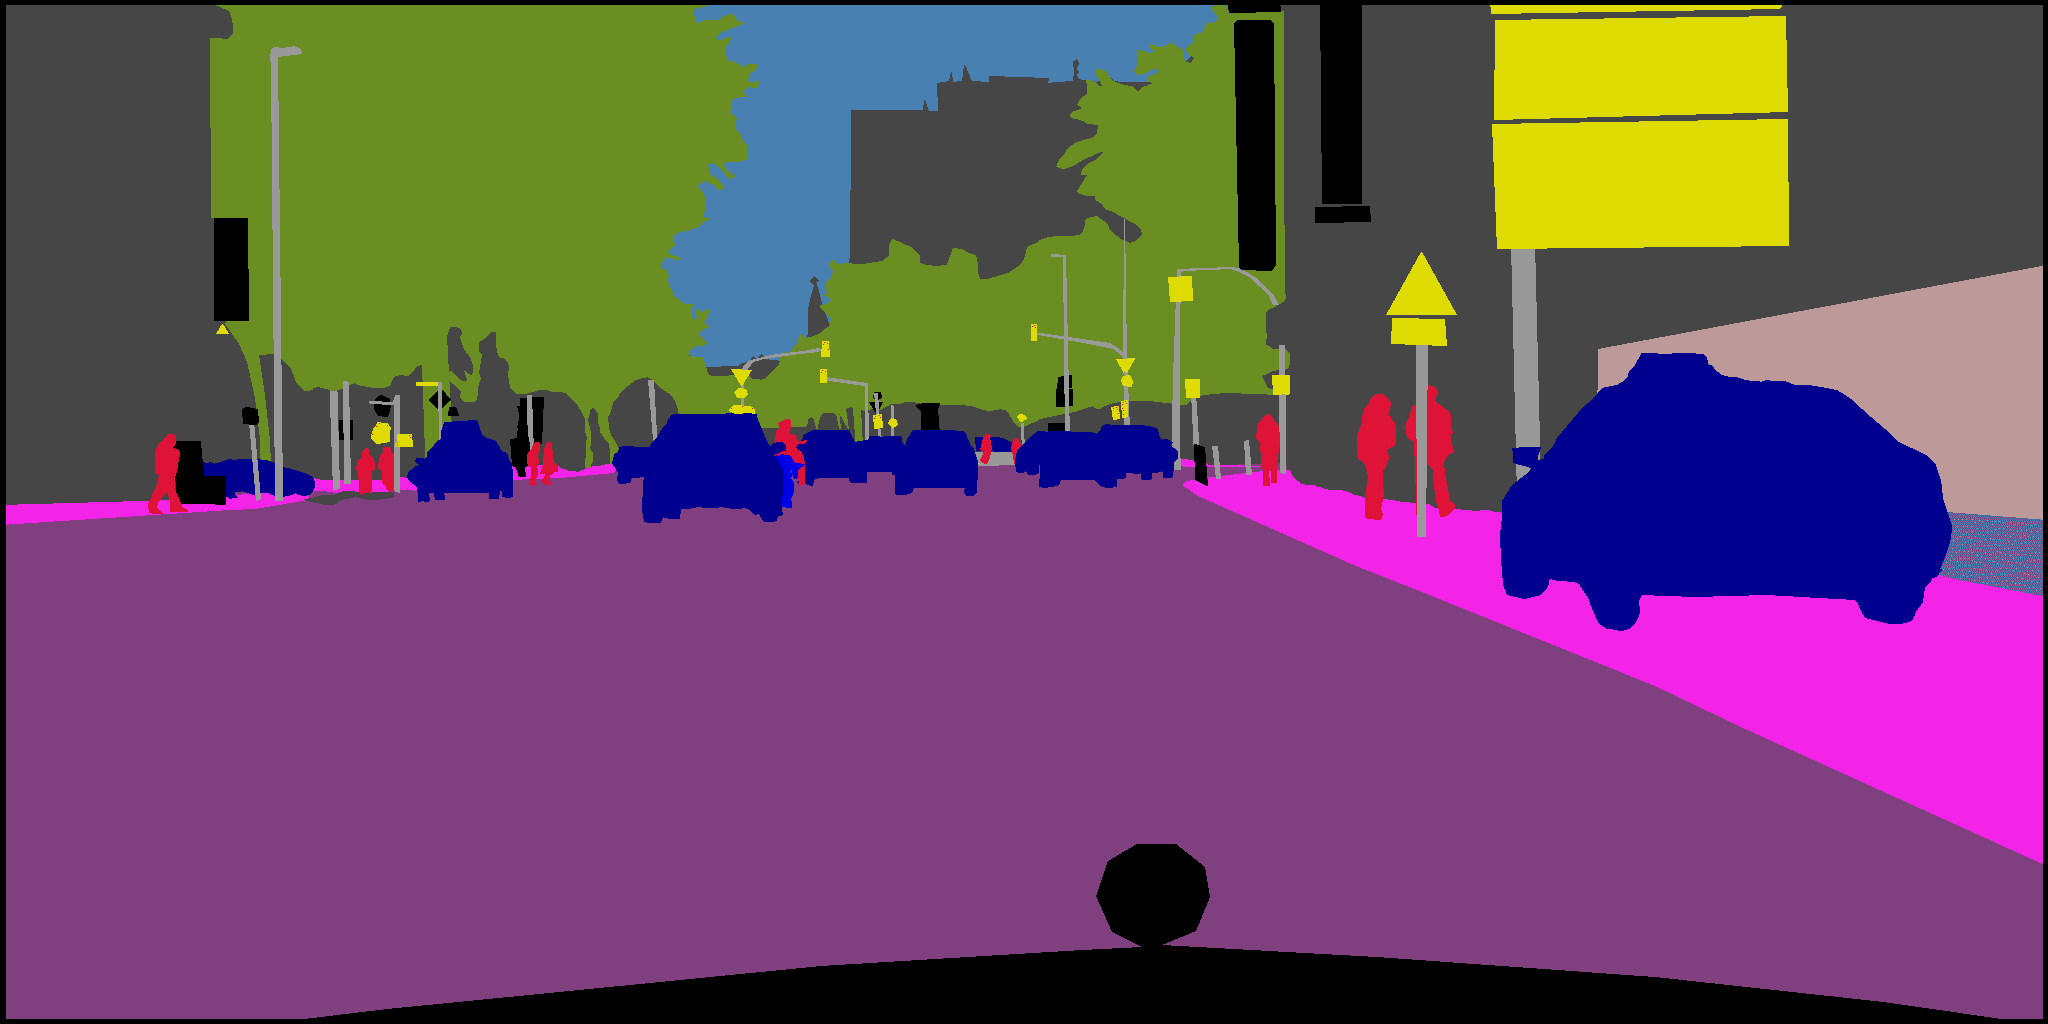
\includegraphics[width=\linewidth, height=0.2\textheight]{Images/Chapter3/aachen_000005_000019_gtFine_color.png}
		\caption{تصویر رنگارنگ}
		\label{f64}
	\end{subfigure}\hfil
	\begin{subfigure}{0.45\textwidth}
		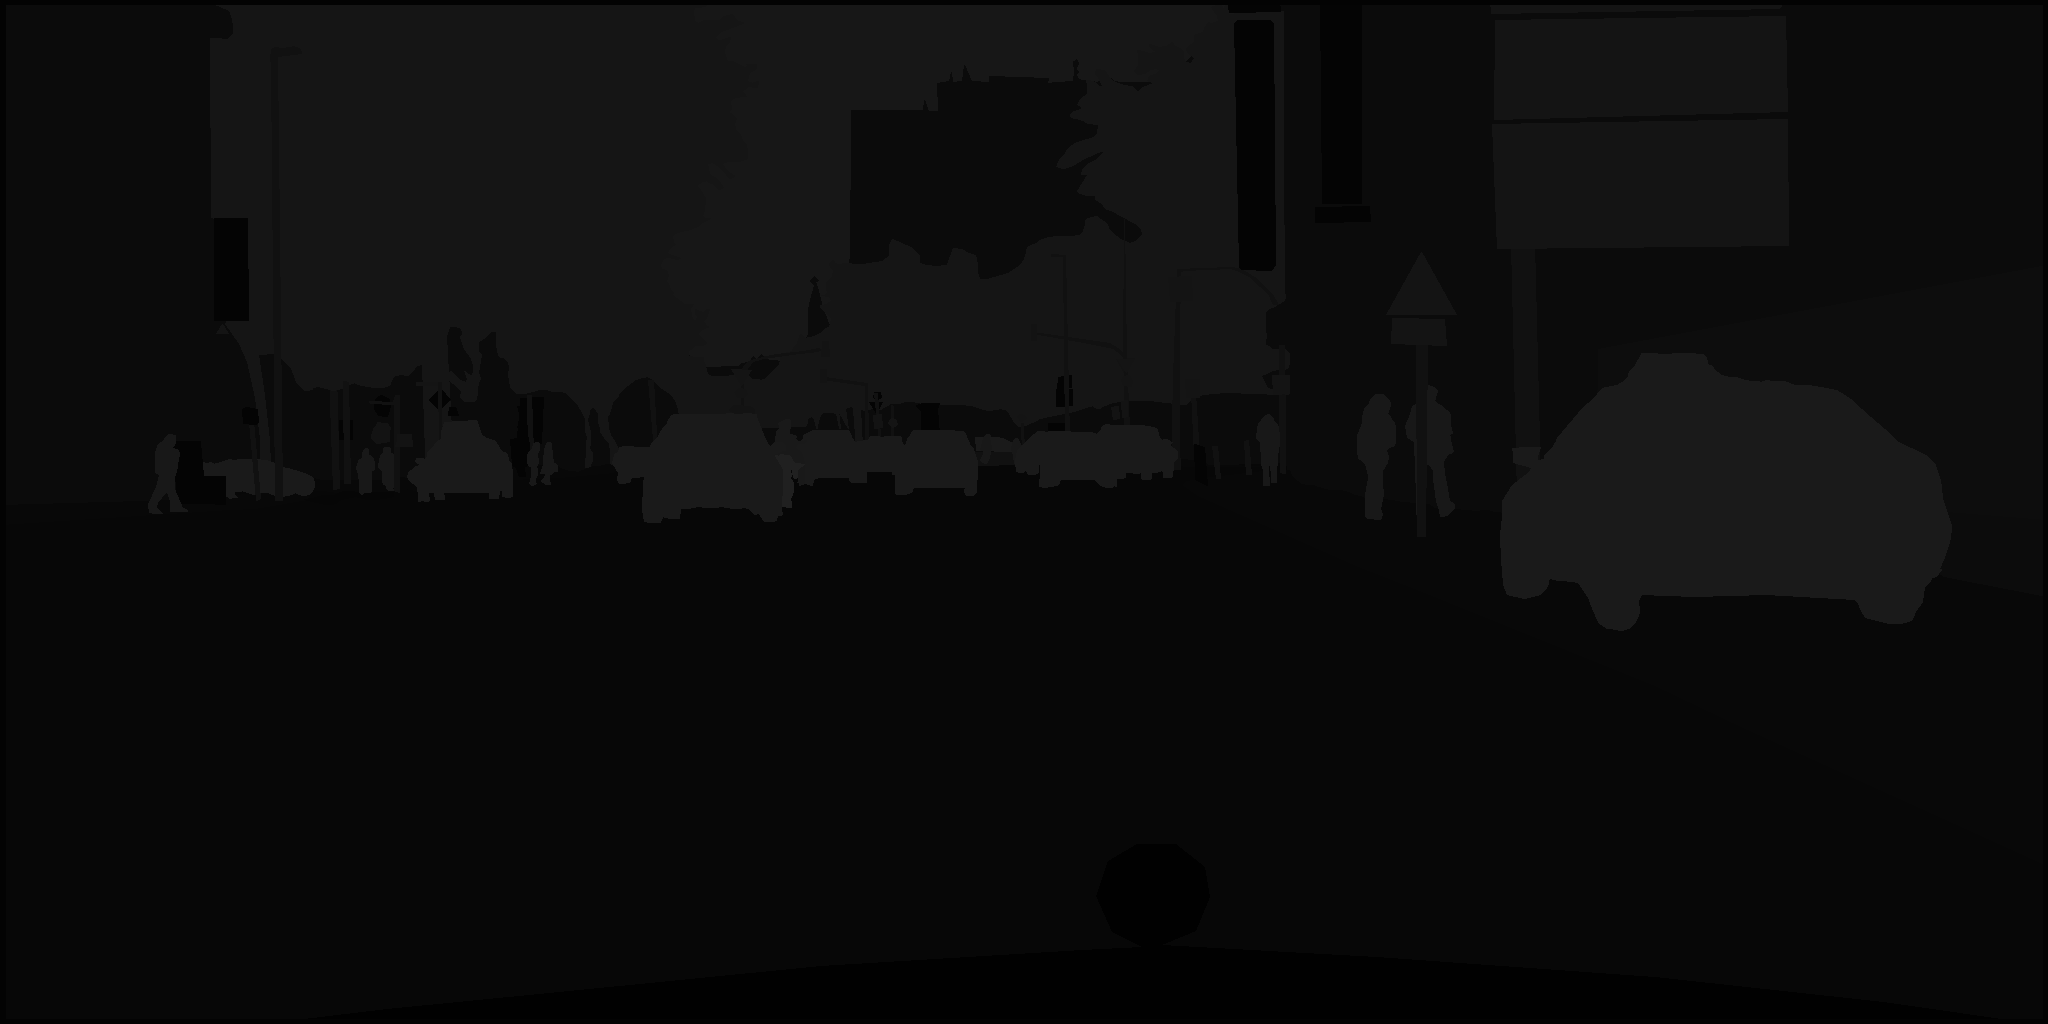
\includegraphics[width=\linewidth, height=0.2\textheight]{Images/Chapter3/aachen_000005_000019_gtFine_labelIds.png}
		\caption{تصویر خاکستری شناسه‌ها}
		\label{f65}
	\end{subfigure}
	\centering
	\caption{نمونه تبدیل نقشه تقسیم‌بندی شده به تصویر رنگارنگ متناظر}
	\label{fig:fig3}
\end{figure}

\section{معماری رمزگذار-رمزگشا}

معماری رمزگذار-رمزگشا
\LTRfootnote{Encoder-decoder}
یک نوع معماری شبکه عصبی است که برای یادگیری توالی به توالی
\LTRfootnote{Sequence to sequence learning}
\cite{sutskever2014sequence}
مورد استفاده قرار می‌گیرد. این معماری شامل دو بخش اصلی، یعنی رمزگذار
\LTRfootnote{Encoder}
و رمزگشا
\LTRfootnote{Decoder}
است که در آن رمزگذار تصویر ورودی را دریافت و پردازش می‌کند تا مجموعه‌ای از بردار‌های ویژگی‌
\LTRfootnote{Feature vectors}
برای تصویر تولید کند. سپس، این بردار‌های ویژگی‌ توسط رمزگشا برای بزرگ‌نمایی تصویر خروجی به اندازه تصویر ورودی استفاده می‌شوند. ایده اصلی پشت این معماری آن است که بتواند یک فرم از داده (در اینجا تصویر) را دریافت کرده و به فرم دیگری (مانند تصویر تقسیم‌بندی معنایی شده معادل) تبدیل کند. با انجام این کار، خودرو قادر خواهد بود که چگونگی ارتباطات بین تصاویر ورودی و خروجی را درک کند.

این معماری می‌تواند در بسیاری از حوزه‌ها مورد استفاده قرار بگیرد، از جمله پردازش تصویر، ترجمه ماشینی
\LTRfootnote{Machine translation}
، تولید متن توسط تصویر
\LTRfootnote{Image to text}
، و غیره. در هر حالت، رمزگذار مسئول استخراج ویژگی‌های مهم از داده ورودی و تولید ویژگی‌های نهان است که اطلاعات اصلی داده را در خود جاسازی می‌کند. سپس، رمزگشا این ویژگی‌های نهان را به فرم دیگری از داده ترجمه می‌کند که معمولاً خروجی مورد نظر است. این معماری به عنوان یکی از روش‌های موثر برای یادگیری مدل‌های پیچیده از داده‌های توالی به توالی شناخته می‌شود و در مسائلی که توالی و ارتباطات بین داده‌ها مهم هستند، بسیار مفید است. در تصویر زیر، این معماری به صورت یک نمودار نشان داده شده است:

\begin{figure}[ht]
	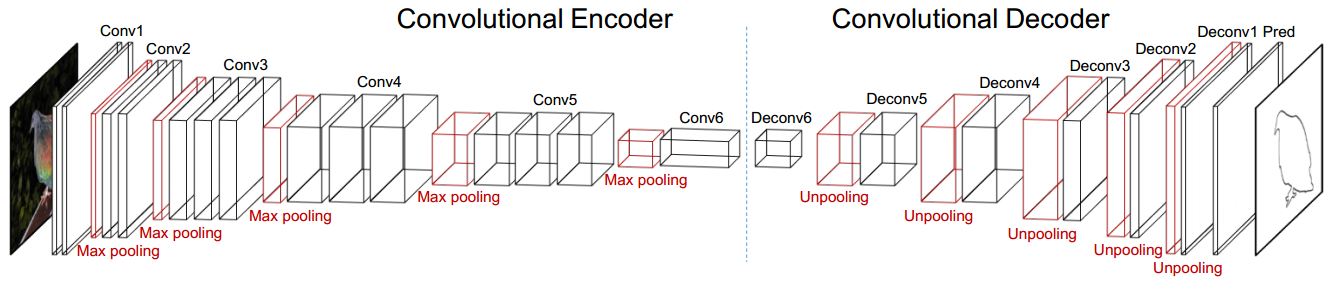
\includegraphics[width=\linewidth, height=0.2\textheight]{Images/Chapter2/encoder-decoder.png}
	\centering
	\caption{معماری رمزگذار-رمزگشا}
	\label{fig:fig4}
\end{figure}

\subsection{شبکه رمزگذار}

رمزگذار، اولین بخش از معماری رمزگذار-رمزگشا است و در پردازش و استخراج اطلاعات از داده ورودی نقش اساسی دارد. این بخش وظیفه استخراج ویژگی‌های معنادار از داده را بر عهده دارد که سپس توسط رمزگشا برای پردازش و بازسازی اطلاعات به فرم دیگر استفاده می‌شود. روشی که فرآیند رمزگذاری کار می‌کند، بسته به نوع کاربرد متفاوت است. در وظایف پردازش تصویر، عموماً از لایه‌های کانولوشنی
\LTRfootnote{Convolutional layers}
به همراه لایه‌های ادغام
\LTRfootnote{Pooling layer}
، فعال‌ساز
\LTRfootnote{Activation function}
و نرمال‌ساز
\LTRfootnote{Normalization}
استفاده می‌شود تا تصویر اصلی به مرور کوچک‌تر شده، اطلاعات اضافی و فضاهای خالی آن حذف شده و در نهایت به تعدادی بردار‌ ویژگی شکسته شود.

لایه‌های کانولوشنی مسئول استخراج ویژگی‌های تصویر ورودی هستند. این لایه‌ها از ویژگی‌های سطح پایین مانند لبه‌ها و رنگ‌ها تا ویژگی‌های سطح بالاتری مانند شکل‌ها و ساختارهای اشیاء را یاد می‌گیرند. هر لایه کانولوشنی مجموعه‌ای از فیلترها را به تصویر ورودی اعمال می‌کند و آن را به بردار‌های ویژگی تبدیل می‌کند که جنبه‌های مختلفی از محتوای تصویر را شامل می‌شود.

لایه‌های ادغام نقشه‌های ویژگی را با حفظ اطلاعات مهم‌تر آن کاهش یا به اصطلاح خلاصه می‌کنند. توابع فعال‌سازی غیرخطی
\LTRfootnote{Non-linear activation functions}
به شبکه این امکان را می‌دهند که روابط پیچیده در داده‌ها آموخته شود. لایه‌های نرمال‌ساز مانند نرمال‌سازی دسته‌ای
\LTRfootnote{Batch normalization}
نیز حساسیت شبکه را به وزن‌های اولیه و نرخ یادگیری
\LTRfootnote{Learning rate}
کاهش می‌دهند و کمک می‌کنند مدل بتواند نرخ‌های یادگیری بالاتری را نیز تحمل کرده و مشکلاتی نظیر انفجار
\LTRfootnote{Exploding gradient descent}
و یا ناپدید شدن گرادیان‌ها
\LTRfootnote{Vanishing gradient descent}
رخ ندهد.

\subsection{شبکه رمزگشا}

رمزگشا، بخش دوم و مهم از معماری رمزگذار-رمزگشا است که مسئول بازسازی بردارهای ویژگی حاصل از رمزگذار و بازسازی آن به شکل اصلی یا شبیه به آن است. این بخش از معماری معمولاً با استفاده از لایه‌های کانولوشنی معکوس
\LTRfootnote{Transposed Convolutional layers}
و یا لایه‌های ادغام معکوس
\LTRfootnote{Unpooling layers}
طراحی می‌شود. برای انجام این کار، باید ارتباطی بین آنچه که رمزگذار شده و آنچه که باید بازسازی شود وجود داشته باشد که عموما در لایه و یا لایه‌هایی بین رمزگذار و رمزگشا به عنوان فضای پنهان
\LTRfootnote{Latent space}
ذخیره می‌شود تا رمزگشا بتواند خروجی معناداری با استفاده از این واحد تولید کند.

از مشکل رایج در معماری رمزگذار-رمزگشا به اندازه بزرگ نبودن فضای پنهان یا بیش از اندازه بزرگ بودن آن است که باعث تولید خروجی ضعیف و یا با جزئیات نامطلوب می‌شود. به عبارت دیگر، اگر فضای پنهان به اندازه کافی بزرگ نباشد، ارتباط بین آنچه رمزگذاری شده و آنچه باید بازسازی شود به طور کامل داخل این ذخیره نشده و در نتیجه نمی‌توان بازسازی معناداری داشته باشیم. در عین حال، اگر فضای پنهان بیش از اندازه بزرگ باشد، الگوهای نامطلوبی توسط مدل کشف شده که متناسب با مساله لزوماً مطلوب ما نیستند.

\section{معماری‌های تقسیم‌بندی معنایی در پزشکی}

در این بخش به مطالعه چند معماری مورد استفاده در مسایل تقسیم بندی معنایی می‌پردازیم.

\subsection{معماری \lr{FCN}}

معماری شبکه کاملا کانولوشنی
\cite{long2015fully}
\LTRfootnote{Fully convolutional network (FCN)}
یک نوآوری بسیار مهم در زمینه تقسیم‌بندی معنایی است که از مدل‌های سنتی شبکه‌های عصبی کانولوشنی با لایه‌های انتهایی کاملا متصل تفاوت دارد. در این معماری، هر پیکسل تصویر به دسته‌های مختلف تقسیم می‌شود، که این امر با استفاده از لایه‌های کانولوشنی و بدون نیاز به لایه‌های کاملاً
\LTRfootnote{Fully connected layer (FC)}
متصل انجام می‌شود. در مدل‌های سنتی‌تر مانند
\verb*|VGG|
\cite{simonyan2014very}
، از لایه‌های کاملاً متصل برای تولید خروجی دسته‌بندی شده استفاده می‌شوند، در حالی که در معماری کاملا کانولوشنی، این لایه‌های کاملاً متصل با لایه‌های کانولوشنی جایگزین می‌شوند. این تغییر باعث می‌شود که شبکه بتواند تصاویر ورودی با ابعاد دلخواه را بپذیرد و خروجی با همان ابعاد تولید کند.

یکی از مزایای این معماری این است که امکان اجرای تقسیم‌بندی معنایی با دقت بالا بدون نیاز به لایه‌های کاملاً متصل فراهم می‌کند. همچنین، اتصالات پرش
\cite{drozdzal2016importance}
\LTRfootnote{Skip Connection}
که در این معماری معرفی شده‌اند، امکان ترکیب اطلاعات معنایی از لایه‌های عمیق با اطلاعات ظاهری از لایه‌های کم عمق را فراهم می‌کنند. این امر منجر به تولید تقسیم‌بندی‌های با جزئیات بیشتر می‌شود که بهبود قابل توجهی در کیفیت و دقت تصویرهای تقسیم‌بندی شده دارد.

\begin{figure}[ht]
	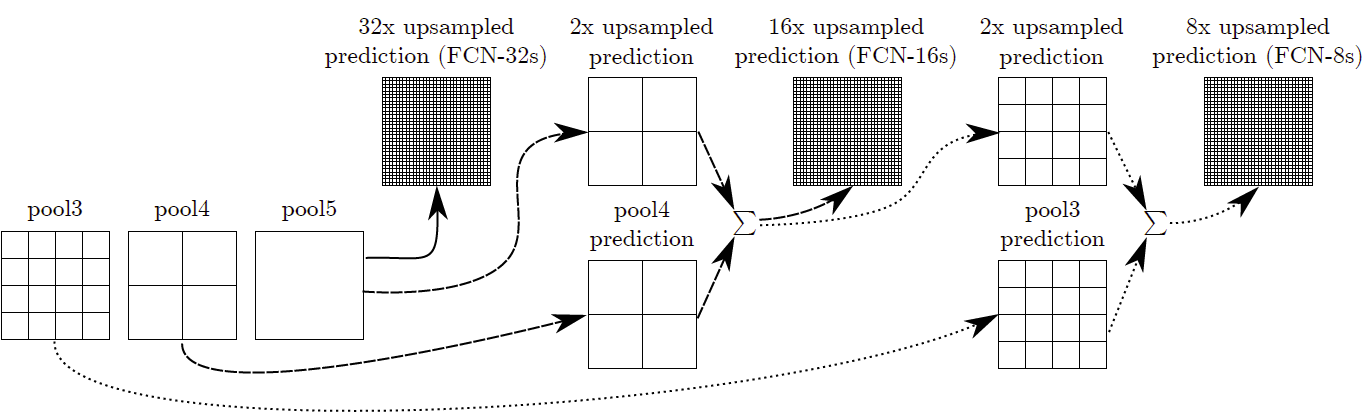
\includegraphics[width=\linewidth, height=0.2\textheight]{Images/Chapter2/FCN.png}
	\centering
	\caption{معماری اتصالات پرش در مدل کاملا کانولوشنی}
	\label{fig:fig5}
\end{figure}

اتصالات پرش یکی از ویژگی‌های کلیدی در شبکه‌های عصبی کانولوشنی
\LTRfootnote{Convolutional Neural Network (CNN)}
هستند که در بسیاری از مسایل تقسیم‌بندی معنایی مورد استفاده قرار می‌گیرند. این اتصالات به شبکه این امکان را می‌دهند که اطلاعات از برخی از لایه‌ها عبور کرده و  مستقیما به لایه‌های بعدی منتقل شوند، در نتیجه جریان مستقیم‌تری از داده دست نخورده به لایه‌های بعدی داشته باشیم.

استفاده همزمان از اتصالات پرش بلند و کوتاه در معماری شبکه‌های عصبی کانولوشنی می‌تواند به بهبود قابل توجهی در دقت تقسیم‌بندی منجر شود. اندازه گام این اتصالات (با اندازه‌های 32، 16 و 8 سلول) مستقیماً بر روی دقت بالانمایی تأثیر می‌گذارد. مدل‌های با گام‌های کوچکتر (در اینجا
\verb*|FCN8|
)، قادرند جزئیات فضایی بیشتری را حفظ کنند و نقشه‌های تقسیم‌بندی دقیق‌تری تولید کنند. اما به همراه این مزیت، گام‌های کوچکتر نیز هزینه محاسباتی
\LTRfootnote{Computational cost}
و زمان استنتاج
\LTRfootnote{Inference time}
را افزایش می‌دهند.

در ارزیابی مدل‌ها با استفاده از شاخص دقت معمولاً مدل‌های با اندازه گام کوچک‌تر عملکرد بهتری را نسبت به مدل‌های مشابه از خود نشان دهند. به عنوان مثال، مدل
\verb*|FCN8|
با مقدار 62.7 در شاخص میانگین اشتراک بر اجتماع
\LTRfootnote{Mean IoU}
عملکرد بهتری را نسبت به مدل‌های مشابه از خود نشان داده می‌دهد.

\subsection{معماری \lr{U-NET}}

معماری
\verb*|U|
-شکل
\cite{ronneberger2015u}
ایده اصلی طرح خود را از شبکه‌های عصبی کانولوشنی می‌گیرد و از آن برای پیش‌بینی پیکسل به پیکسل
\LTRfootnote{Pixel-to-pixel}
در تقسیم‌بندی معنایی استفاده می‌کند. این معماری محدودیت‌های معماری‌های سنتی را برای وظایف تقسیم‌بندی معنایی از بین می‌برد. بر خلاف شبکه‌های عصبی کانولوشنی استاندارد که از لایه‌های کاملاً متصل برای تولید خروجی تصنیفی استفاده می‌کنند، معماری 
\verb*|U|
-شکل، مشابه معماری
\verb*|FCN|
، یک شبکه کاملاً کانولوشنی است که می‌تواند تصاویر ورودی با ابعاد دلخواه را بپذیرد و نقشه‌های تقسیم‌بندی با همان ابعاد تصاویر ورودی را تولید کند.

این مدل نیز از معماری رمزگذار-رمزگشا پیروی کرده که شکلی مانند حرف
\verb*|U|
انگلیسی را تشکیل می‌دهند. در بخش رمزگذار، از کانولوشن‌های تکراری و لایه‌های ادغامی برای یادگیری ویژگی‌های سلسله‌مراتبی استفاده می‌شود. در بخش رمزگشا، ویژگی‌ها بالا‌نمایی می‌شوند و با ویژگی‌های برخی از لایه‌های رمزگذار از طریق اتصالات پرش ترکیب می‌شوند. عموما مدل‌های
\verb*|U|
-شکل از معماری رمزگذار-رمزگشا متقارن
\LTRfootnote{Symmetric encoder-decoder architecture}
\cite{mao2016image}
استفاده می‌کنند که به معنای مشابه بودن این دو بخش دو تعداد لایه‌ها و مشخصات هر لایه بوده، با این تفاوت که عکس یکدیگر عمل می‌کنند.

نوآوری اصلی در معماری
\verb*|U|
-شکل، استفاده کارآمد از اتصالات پرش و توانایی تولید خروجی‌های با وضوح بالا، حتی با مجموعه داده آموزشی نسبتاً کوچک است. اتصالات پرش به شبکه امکان می‌دهند جزئیات ویژگی‌های رمزگذار و رمزگشا را ترکیب کنند و نقشه‌های تقسیم‌بندی دقیق‌تری تولید کنند. این معماری همچنین بازسازی بهتری روی لبه‌های اشیا انجام می‌دهد.

\begin{figure}[ht]
	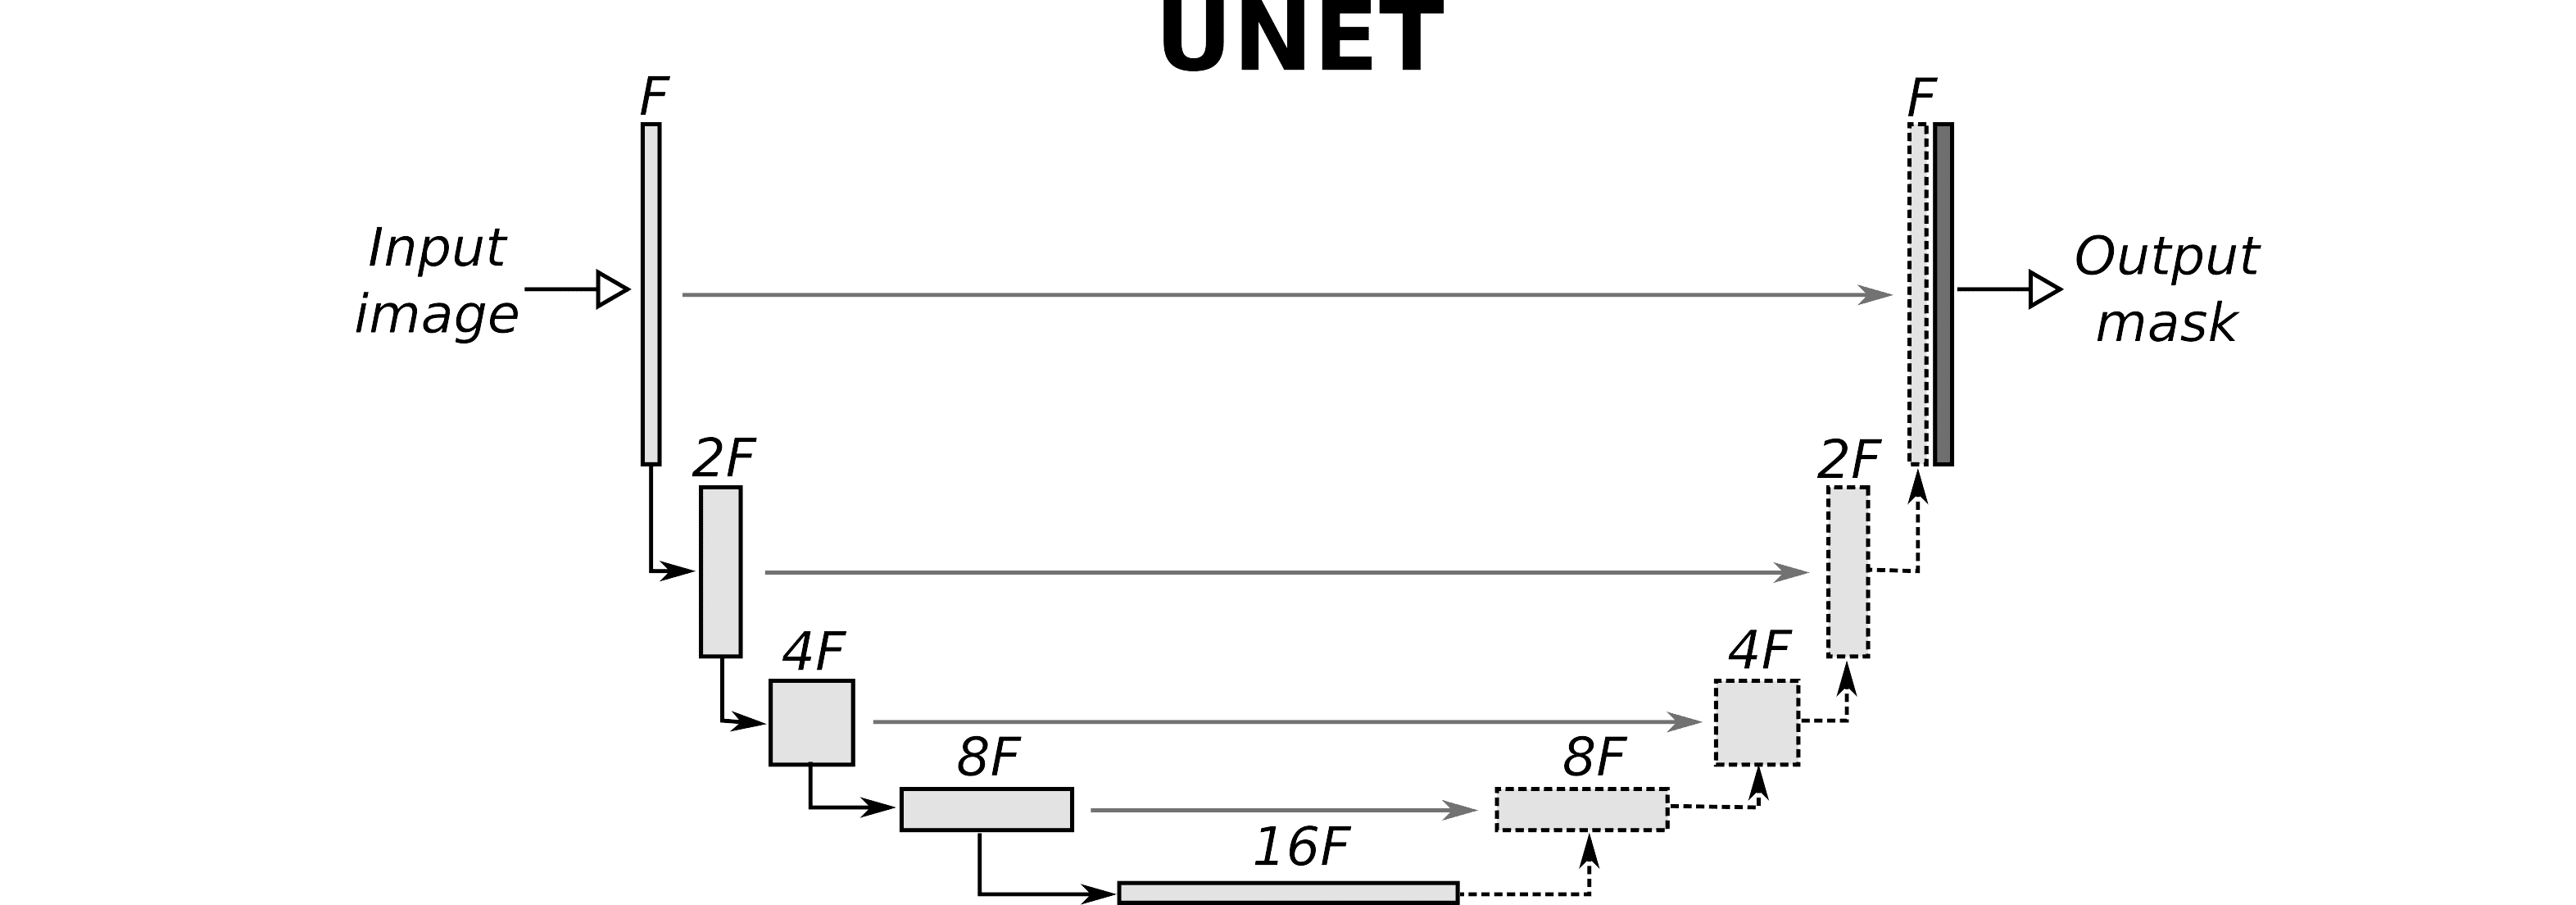
\includegraphics[width=\linewidth, height=0.2\textheight]{Images/Chapter2/UNET.png}
	\centering
	\caption{معماری مدل \lr{U}-شکل}
	\label{fig:fig6}
\end{figure}

\section{خلاصه}

به طور کلی، معماری‌های رمزگذار-رمزگشا به طور قابل توجهی رویکرد حل مسایل تقسیم‌بندی معنایی را تغییر داده‌اند. این معماری‌ها از توانایی‌های شبکه‌های عصبی کانولوشنی برای پیش‌بینی دقیق پیکسل به پیکسل بهره می‌برند و به وجود آوردن نقشه‌های تقسیم‌بندی دقیق و جزئی‌تر کمک می‌کنند. با استفاده از تکنیک‌هایی مانند اتصالات پرش و بالانمایی، ساختار رمزگذار-رمزگشا قادر است جزئیات فضایی و اطلاعات معنایی را با دقت بالاتر در نظر بگیرد و نقشه‌های تقسیم‌بندی دقیق‌تری را تولید کند.
با این حال، معماری‌های
\verb*|FCN|
و
\verb*|U|
-شکل هر کدام ویژگی‌ها و مزایای خود را دارند. معماری U-شکل به دلیل ساختار رمزگذار-رمزگشا تقارنی و استفاده گسترده از اتصالات پرش، نسبت به
\verb*|FCN|
برتری دارد. طراحی منحصر به فرد این مدل به آن امکان می‌دهد که حتی با مجموعه داده‌های آموزشی محدود، خروجی‌های تقسیم‌بندی با وضوح بالا را تولید کند، به‌ ویژه در وظایفی که دقت به جزئیاتی نظیر لبه‌ها حیاتی است، مانند تقسیم‌بندی تصاویر پزشکی. از سوی دیگر،
\verb*|FCN|
رویکردی انعطاف‌پذیرتر را ارائه می‌دهد و ممکن است در مواردی که کارآیی محاسباتی یا مجموعه داده‌های آموزشی بزرگ اولویت دارند، ترجیح داده شود. به طور خلاصه، انتخاب بین این دو معماری بسته به نیازها و شرایط خاص هر پروژه است. با این حال هر دو از سرعت پایینی در زمان استنتاج برخورداند که آن‌ها را برای پردازش لحظه‌ای مناسب نمی‌سازد.


\chapter{روش‌های پیشنهادی}

\section{معماری رمزگذار-رمزگشا}

در فصل پیشین، مرور کار‌های مرتبط، به توضیح مفاهیم پرداخته و به چندین مدل کارآمد در مسایل تقسیم‌بندی معنایی اشاره کردیم. بزرگ‌ترین اشکال استفاده از مدل های ذکر شده برای پردازش آنی، سرعت پایین آنها بوده که در استفاده برای خودرو‌های خودران چالش‌برانگیز می‌شود. در این فصل به طور مفصل به بررسی چندین مدل پیشنهادی برای تقسیم‌بندی معنایی که بخصوص برای پردازش آنی در خودرو‌های خودران طراحی شده اند می‌پردازیم.

\subsection{مدل \lr{SQNet}}

از راهکار های ساده برای بهبود عملکرد اکثر مدل های یادگیری عمیق که برای حل مسایل، افزایش اندازه شبکه است. این راهکار در حوزه تقسیم‌بندی معنایی نیز منجر به بوجود آمدن معماری های نوین مانند شبکه های مولد
\LTRfootnote{Generative Adversarial Networks (GAN)}
و مدل‌های انتشاری
\LTRfootnote{Diffusion Model}
شده است که به دلیل دقت بالا عموما در حوزه پزشکی مورد استفاده قرار می‌گیرند، اما به دلیل سرعت پایین آن‌ها در حوزه خودرو‌های خودران عملکرد خوبی از خود نشان نمی‌دهند. استفاده از این شبکه‌های دقیق اما بزرگ برای خودروهای خودران به‌طور کلی غیرقابل اجرا یا حداقل با دشواری و هزینه بسیار زیادی همراه است. پس تمرکز به سوی بهینه‌تر کردن مدل ها و استفاده از روش های نوین برای رسیدن به دقت مشابه و سرعت بیشتر تغییر کرده است، زیرا در خودرو‌های خودران قدرت پردازش و زمان کافی حائز اهمیت است. پس عمده مدل‌های معرفی شده به نوعی به معاوضه بین دقت و سرعت پرداخته و در تلاش هستند که با کمترین از دست رفت دقت بتوان سرعت پردازش را بالا برد.

تحقیقات گسترده ای بر روی کاهش توان پردازش مورد نیاز برای تقسیم‌بندی معنایی در خودرو‌های خودران صورت گرفته است. برای مثال معماری
\verb*|SqueezeNet|
\cite{iandola2016squeezenet}
نشان داد که با استفاده از یک معماری موثرتر که در آن از کانولوشن‌های تک واحدی برای فشرده کردن اطلاعات بکار گرفته شده، می‌توان همان دقت در پردازش تصاویر را با استفاده از ۵۰ برابر تعداد وزن‌های کمتر ایجاد نمود. همچنین با تغییر مولفه‌های جزئی‌تری مانند توابع ‌فعال‌ساز و یا حذف لایه‌هایی نظیر نرمال‌ساز می‌توانند در افزایش سرعت موثر باشند. مدل
\verb*|SQNet|
\cite{treml2016speeding}
که نیز از معماری رمزگذار-رمزگشا
\LTRfootnote{Encoder-Decoder Architecture}
استفاده می کند، توانسته است با استفاده از این‌گونه تغییرات به پردازش تقریبا آنی دست یابند.

معماری رمزگذار، مشابه آنچه در
\verb*|SqueezeNet|
آمده طراحی شده که ویژگی قابل توجه آن تعداد وزن‌های کمتر آن است که منجر به سرعت گرفتن پردازش آن می‌شود. بخش محاسباتی اصلی در این معماری آتش
\LTRfootnote{Fire module}
نامیده می‌شود که شامل سه عمل کانولوشن به همراه دو تابع‌فعال‌ساز می‌باشد. توابع‌فعال‌ساز یکسوساز
\LTRfootnote{Rectified linear unit (ReLU)}
با توابع‌فعال‌ساز واحد نمایی خطی
\LTRfootnote{Exponential linear unit (ELU)}
جایگزین شده‌اند که بار ‌محاسباتی کمتری داشته، و در عین حال اطلاعات منفی همچنان انتقال پیدا می‌کنند. در رمزگذار از هشت واحد آتش و سه لایه ادغام برای کاهش ابعاد تصویر استفاده شده است.

\begin{figure}[ht]
	\begin{subfigure}{\textwidth}
		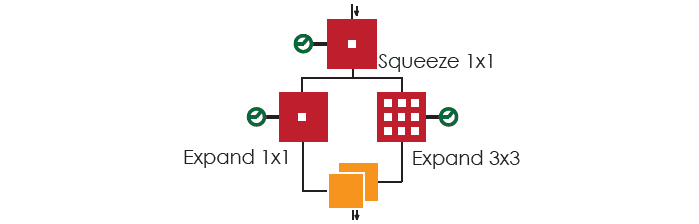
\includegraphics[width=\linewidth, height=0.2\textheight]{Images/Chapter3/SQNet_fire.png}
		\caption{واحد آتش}
		\label{f64}
	\end{subfigure}
	\begin{subfigure}{0.45\textwidth}
		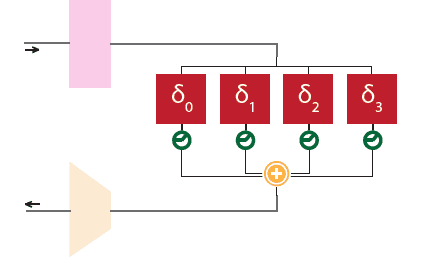
\includegraphics[width=\linewidth, height=0.2\textheight]{Images/Chapter3/SQNet_PDC.png}
		\caption{لایه کانولوشی موازی}
		\label{f65}
	\end{subfigure}
	\begin{subfigure}{0.45\textwidth}
		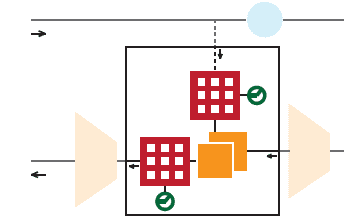
\includegraphics[width=\linewidth, height=0.2\textheight]{Images/Chapter3/SQNet_BRM.png}
		\caption{واحد تصحیح}
		\label{f65}
	\end{subfigure}
	\centering
	\caption{اجزاء معماری \lr{SQNet}}
	\label{fig:fig8}
\end{figure}

رمزگشا بر اساس یک لایه‌های
\verb*|parallel|
\verb*|dilated|
\verb*|convolutions|
مبتنی است که نقشه ویژگی‌ها را در خروجی رمزگذار در اندازه‌های میدان تاثیر مختلف ترکیب می‌کند. این واحد این کار را با استفاده از چهار کانولوشن با اندازه کرنل 3 انجام می‌دهد که معادل نمونه‌برداری لایه ورودی با نرخ‌های مختلف است. در نهایت خروجی چهار کانولوشن را با جمع زدن با یکدیگر با هم ادغام می‌کنیم که باعث می‌شود اندازه میدان دید در ورودی رمزگشا افزایش یابد. این کار باعث می‌شود نسبت به شبکه های تماما متصل، تعداد وزن‌های قابل توجه کمتری را داشته باشیم در حالی که عملکرد مدل حفظ می‌شود.

لایه‌های ادغامی داخل رمزگذار برای اطمینان از پایا بودن
\LTRfootnote{Translation Invariant}
در انتقالات استفاده می‌شوند. با این حال، این لایه‌ها به مرور زمان باعث کاهش وضوح تصویر می‌شوند، چراکه هر بار برخی از اطلاعات تصویر خلاصه یا حذف می‌شود. کانولوشن‌های معکوس
\LTRfootnote{Transposed Convolutions}
در رمزگشا برای افزایش ابعاد تصویر خارج شده از رمزگذار به اندازه اصلی استفاده می‌شوند. در حالت عادی، این معماری قدرت بازسازی بهینه‌ای نداشته و برخی اطلاعات تصویر اصلی از دست خواهد رفت که شدت آن به میزان استفاده از تعداد لایه های ادغامی و شدت کوچک‌نمایی تصویر دارد. برای کمرنگ‌تر کردن این مشکل، فقط از داده‌هایی که مستقیماً از لایه کانولوشن معکوس پیشین می‌آیند استفاده نمی‌کنیم، بلکه آن‌ها با دانش سطح پایین از لایه‌های زیرین رمزگذار ترکیب می‌شود. این کار به تشخیص ساختارهای با وضوح بالاتر کمک می‌کند که در تمیز کردن بهتر مرزهای اشیاء موثر است. پس از محاسبه کانولوشن‌های لایه فعلی و زیرین، هر دو ویژگی بدست آمده با یکدیگر ترکیب شده و سپس بزرگ‌نمایی می‌شود که به این واحد ها اصطلاحا واحد تصحیح
\LTRfootnote{Refinement Module}
گفته می‌شود. پیش‌تر اشاره شد که توابع‌فعال‌ساز متفاوتی برای رمزگذار استفاده می‌شود. این تابع‌ فعال‌ساز برای بخش رمزگشا نیز به همین نحو استفاده می‌شود.

\subsection{مدل \lr{ENet}}

معماری‌های متعددی برای حل مسایل تقسیم‌بندی معنایی مطرح شده‌اند که
\verb*|FCN|
و
\verb*|SegNet|
\cite{badrinarayanan2017segnet}
دو مدل مطرح در این حوزه هستند. از آنجایی که هر دو معماری بر اساس معماری پایه
\verb*|VGG|
طراحی شده‌اند، تعداد پارامتر‌ها و زمان استنتاج بالایی دارند و برای استفاده در حوزه‌هایی که نیاز به پردازش سریع و یا سخت‌افزار ضعیفی دارند مناسب نیستند. مدل
\verb*|ENet|
\cite{paszke2016enet}
\LTRfootnote{Efficient Neural Network}
با هدف پردازش سریع‌تر و دقت بالا طراحی شده است که نیز از معماری رمزگذار-رمزگشا استفاده می‌کند. 

معماری
\verb*|ENet|
از چندین بلوک تشکیل شده. بلوک ابتدایی
\LTRfootnote{Initial block}
شامل یک لایه ادغام حداکثری با پنجره‌‌های 2×2 بدون همپوشانی و یک لایه کانولوشنی با 13 فیلتر است که تصویر را به 16 نقشه ویژگی تبدیل می‌کند. هدف استفاده از این بلوک، کاهش ابعاد تصویر و تبدیل آن به بردار‌های ویژگی است تا اطلاعات غیرمرتبط تصویر حذف شده و بار محاسباتی کاهش پیدا کند. بلوک گلوگاه از اجزای کلیدی این معماری است که به طور مکرر در بخش های مختلف این معماری شاهد آن هستیم.

\begin{figure}[ht]
	\begin{subfigure}{0.45\textwidth}
		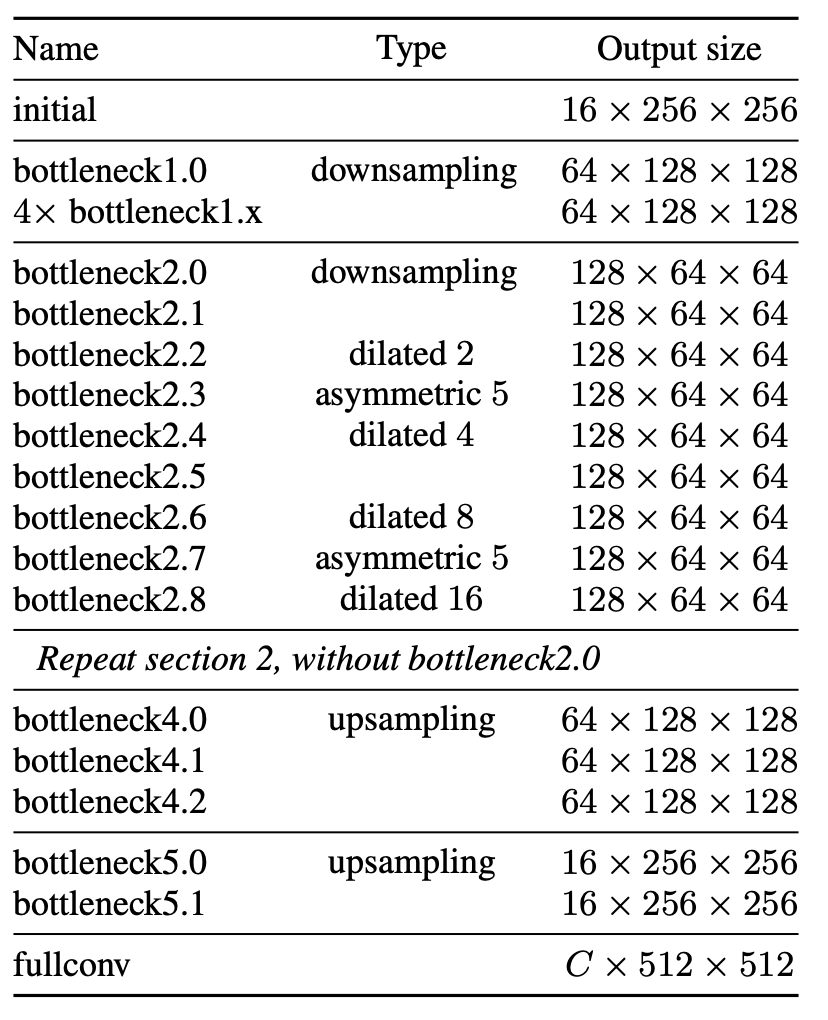
\includegraphics[width=\linewidth, height=0.3\textheight]{Images/Chapter3/ENet.png}
		\caption{معماری کلی شبکه \lr{ENet}}
		\label{f64}
	\end{subfigure}\hfil
	\begin{subfigure}{0.45\textwidth}
		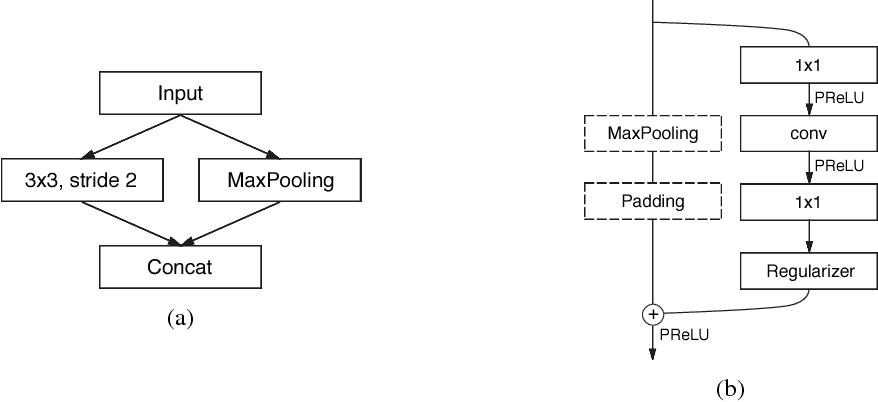
\includegraphics[width=\linewidth, height=0.2\textheight]{Images/Chapter3/ENet_blocks.png}
		\caption{معماری بلوک های شبکه \lr{ENet}}
		\label{f65}
	\end{subfigure}
	\centering
	\caption{نمونه تبدیل نقشه تقسیم‌بندی شده به تصویر رنگارنگ متناظر}
	\label{fig:fig7}
\end{figure}

نمونه‌برداری کاهشی
\LTRfootnote{Downsampling}
به طور کلی منجر به از دست رفتن برخی از اطلاعات داخل تصویر می‌شود و انجام آن بخصوص به صورت مکرر و با ضریب بزرگ به ضرر مدل است. اما از طرفی کاهش ابعاد تصویر به مصرف حافظه کمتر و کاهش بار محاسباتی و تعداد پارامتر های مدل کمک شایانی می‌کند. استراتژی استفاده شده در این معماری بدین گونه است که نمونه‌برداری کاهشی به کمترین تعداد ممکن و در ابتدای مدل انجام شود. مزیت انجام این‌کار در اول مسیر آن است که از پردازش تصاویر با ابعاد بزرگ که هزینه پردازش بالایی دارند جلوگیری می‌شود. برای سرعت بخشیدن به این فرآیند، عملیات ادغام به همراه یک کانولوشن به صورت موازی انجام شده و بردار‌های ویژگی حاصل با یکدیگر ترکیب می‌شوند.

بهینه سازی دیگر بر روی تابع‌فعالساز است. به گونه‌ای که در تمام مدل تابع فعالساز توابع‌فعال‌ساز یکسوساز پارامترسازي شده
\LTRfootnote{Parameterized ReLU (PReLU)}
جایگزین توابع‌فعال‌ساز یکسوساز شده است. این تابع‌فعالساز شیب منفی قابل آموزش دارد که به مدل انعطاف‌پذیری بیشتر و عملکرد بهتری داشته باشیم.

در آخر، استفاده از کانولوشن‌های گسترده
\LTRfootnote{Dilated convolutions}
نوعی دیگر از عملیات کانولوشن هستند که در آن‌ها فاصله‌ بین پیکسل‌های ورودی افزایش می‌یابد. در واقع، این نوع از کانولوشن‌ها به ورودی‌ها اعمال می‌شوند با استفاده از یک فیلتر کانولوشن با فضای پیکسل‌های بزرگ‌تر از یک باعث می‌شود اطلاعات بیشتری از ورودی‌ها در نظر گرفته شود. این نوع از کانولوشن‌ها معمولاً این امکان را برای شبکه فراهم می‌کنند تا بدون افزایش تعداد پارامترها میدان تاثیر بزرگ‌تری داشته باشد.

\section{معماری دو-شاخه}

\subsection{مدل \lr{Fast-SCNN}}

به مرور، تمایل به استفاده از معماری دو-شاخه
\LTRfootnote{Two-branch architecture}
در مدل‌های مطرح شده برای تقسیم‌بندی معنایی سریع افزایش یافته است؛ به طوری که دو شبکه با عمق های متفاوت بر روی تصویر با وضوح‌های متفاوت عمل کرده و در نهایت هر دو شاخه با یکدیگر ترکیب می‌شوند. این معماری اجازه می‌دهد تا در یک شاخه از شبکه‌ای عمیق
\LTRfootnote{Deep network}
بر روی تصویر با وضوح پایین استفاده شود تا اطلاعات اشیاء استخراج و آموخته شود و در شاخه دیگر شبکه‌ای کم عمق
\LTRfootnote{Shallow network}
بر روی همان تصویر اما با وضوح بالاتر به کار گرفته شود تا دقت نهایی تصویر خروجی بهبود یابد. از آنجایی که عمق شبکه و ابعاد تصویر اولیه به طور مستقیم بر روی سرعت پردازش تاثیرگذار هستند، معماری دو-شاخه بهینه‌سازی‌هایی برای پردازش سریع‌تر نسبت به معماری رمزگذار-رمزگشا دارد. مدل
\verb*|Fast|-\verb*|SCNN|
از ۴ بخش تقسیم شده که به صورت سری به یکدیگر متصل شده اند. در ادامه به معرفی اجزای مورد استفاده در این مدل می‌پردازیم.

\begin{figure}[ht]
	\centering
	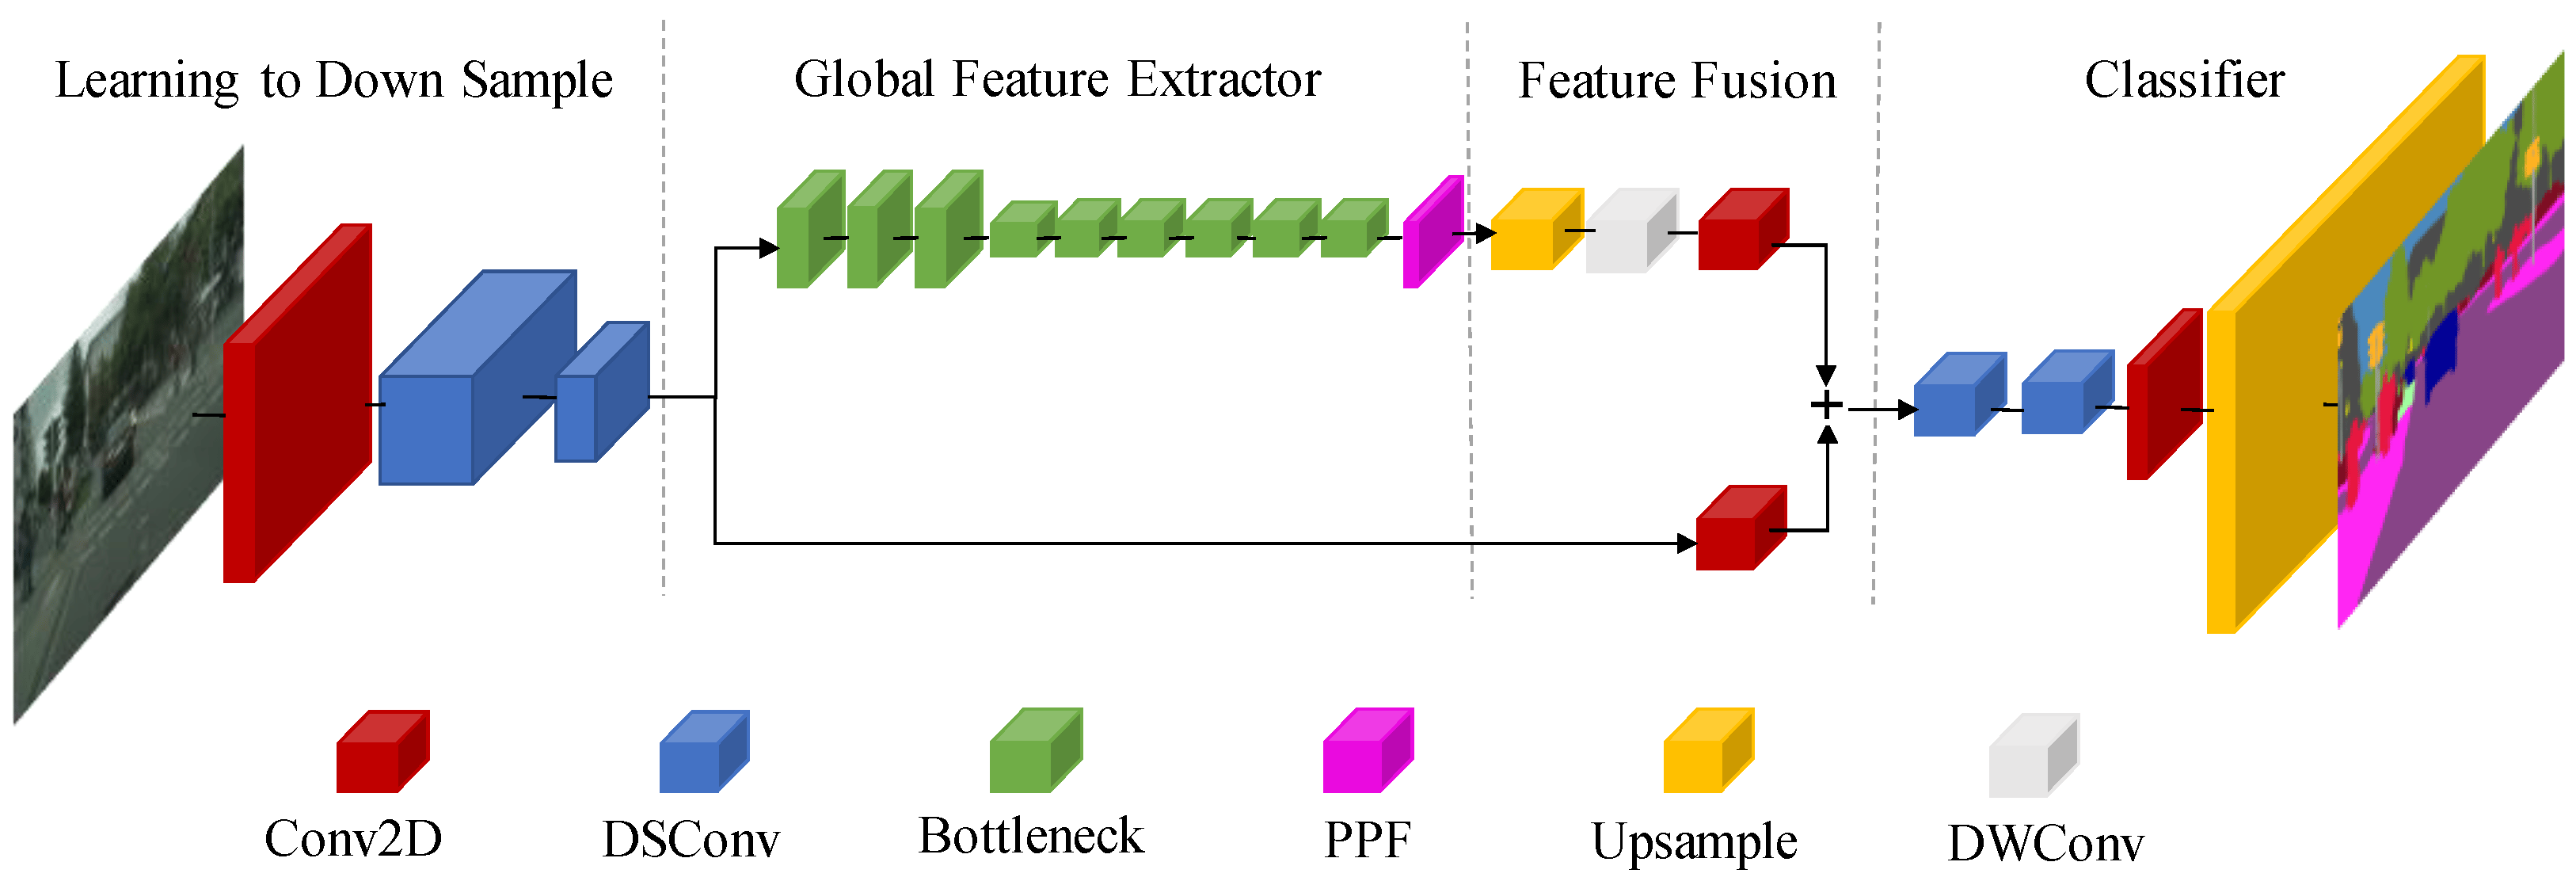
\includegraphics[width=0.9\linewidth, height=0.2\textheight]{Images/Chapter3/FastSCNN.png}
	\caption{معماری مدل \lr{Fast-SCNN}}
	\label{fig:fig10}
\end{figure}

\subsubsection{لایه‌ کانولوشنی تفکیک‌پذیر عمق‌محور}

در یک کانولوشن استاندارد بر روی تصاویر رنگی که عموما ۳ کانال رنگ دارند اینگونه انجام می‌شود که فیلتر به اندازه عمق رنگ ورودی اعمال شده و به ما امکان می‌دهد که کانال‌های رنگی را ترکیب کرده و آن‌ها را کم یا زیاد کنیم. به عبارتی اگر بخواهیم یک تصویر با ابعاد (۳،۱۲،۱۲) را به (۲۵۶،۸،۸) تبدیل کنیم به ۲۵۶ کرنل با ابعاد (۳،۵،۵) نیاز خواهیم داشت که در مجموع کمی بیش از یک میلیون عملیات ضرب خواهیم داشت.

در عملیات کانولوشنی عمق‌محور
\LTRfootnote{Depthwise Convolution}
، هر فیلتر به صورت جداگانه بر روی هر کانال اعمال شده و در نتیجه تعداد کانال‌های تصویر ثابت می‌ماند. به عبارتی، در تبدیل تصویر با ابعاد مشابه به ابعاد ثانوی (۳،۸،۸) نیاز به ۳ کرنل (به تعداد کانال‌های تصویر) با ابعاد (۱،۵،۵) داریم که در مجموع تقریبا ۵۰۰۰ عملیات ضرب می‌شود. سپس برای افزایش تعداد کانال‌های تصویر به عملیات کانولوشن نقطه‌محور
\LTRfootnote{Pointwise Convolution}
\cite{hua2018pointwise}
نیاز خواهیم داشت. برای مثال افزایش تعداد کانال‌های تصویر از ۳ به ۲۵۶ نیازمند ۲۵۶ کرنل با ابعاد (۳،۱،۱) دارد که در مجموع ۵۰۰۰۰ عملیات ضرب می‌شود. در نهایت ترکیب این دو لایه که لایه‌ کانولوشنی تفکیک‌پذیر عمق‌محور
\LTRfootnote{Depthwise Separable Convolutions}
\cite{chollet2017xception, nascimento2019dsconv}
نام دارد، معادل عملیات کانولوشن استاندارد می‌شود. لایه جدید در تئوری ۲۵ برابر و در عمل ۲ الی ۸ برابر سریع تر از کانولوشن استاندارد است.

\begin{figure}[ht]
	\centering
	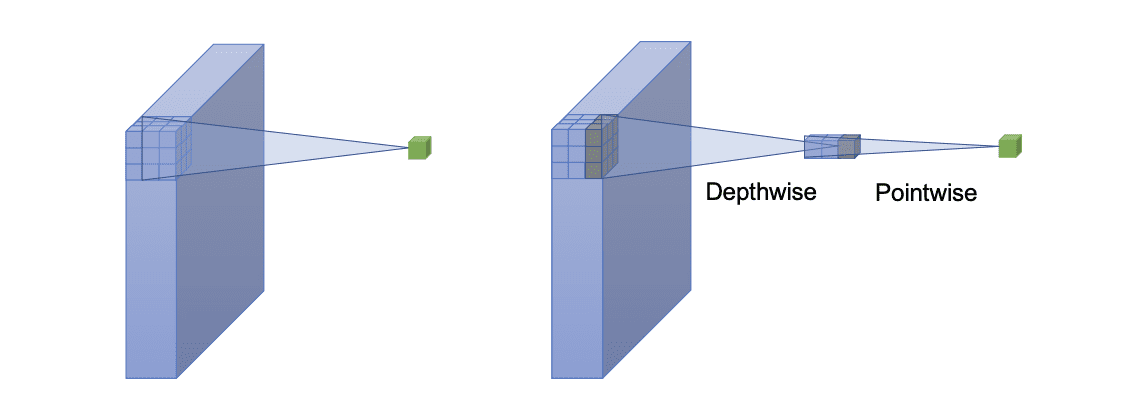
\includegraphics[width=0.9\linewidth, height=0.2\textheight]{Images/Chapter3/DepthwiseSeparableConvolution.png}
	\caption{مقایسه کانولوشن استاندارد و تفکیک‌پذیر عمق‌محور}
	\label{fig:fig9}
\end{figure}

\subsubsection{بخش \lr{learning to downsample}}

این اولین بخش از معماری
\verb*|Fast|-\verb*|SCNN|
است که از سه لایه اصلی تشکیل شده است که اولین آنها لایه کانولوشنی استاندارد است و دو جزء دیگر لایه‌های کانولوشنی تفکیک‌پذیر عمق‌محور که پیش‌تر معرفی شدند نام دارند. لایه‌های کانولوشنی تفکیک‌پذیر عمق‌محور در حالت عادی به لحاظ محاسباتی کارآمدتر هستند، اما برای اولین لایه از لایه کانولوشن استاندارد استفاده می‌کنیم زیرا برتری محاسباتی این لایه در اولین لایه به دلیل تنها ۳ کاناله بودن تصویر بیشتر است. پس از تمامی لایه‌های اصلی از نرمال‌سازی دسته‌ای و تابع‌فعال‌ساز
\verb*|ReLU|
استفاده شده است. معماری این بخش در شکل
\ref{fig:fig10}
قابل مشاهده است.

\subsubsection{بخش استخراج ویژگی‌های سراسری}

بخش استخراج ویژگی‌های سراسری
\LTRfootnote{Global feature extractor}
به دنبال استخراج اطلاعات از فضای تصویر برای تقسیم‌بندی است. تصویر ورودی این جزء، خروجی مستقیم بخش
\verb*|learning to downsample|
است که معادل یک هشتم ابعاد تصویر اصلی را دارد. این کوچک‌نمایی در عین کاهش میزان محاسبات، اکثر جزئیات مهم تصویر را حفظ می‌کند. در این بخش از تعدادی لایه بلوک اضافی گلوگاه
\LTRfootnote{Bottleneck residual block}
استفاده می‌شود که در آنها لایه کانولوشنی تفکیک‌پذیر عمقی جایگزین لایه‌های کانولوشنی عادی شده تا تعداد وزن‌های مورد استفاده در هر بلوک و در نتیجه تعداد عملیات برای محاسبه خروجی کاهش یابد. در آخر از لایه ادغام هرمی
\LTRfootnote{Pyramid pooling module (PPM)}
\cite{zhao2017pyramid}
استفاده شده که تا اطلاعات موجود در تصویر در مقیاس‌های مختلف تجمیع شوند که با استفاده از آنها پس از بلوک های اضافی گلوگاه تاثیر مثبتی بر روی خروجی می‌گذارد. نمای کلی این بخش در شکر 
\ref{fig:fig10}
قابل مشاهده است.

\subsubsection{گذاخت ویژگی‌ها و دسته‌بندی}

در بخش گداخت ویژگی‌ها
\LTRfootnote{Feature fusion module}
، از جمع ویژگی‌های به دلیل بهره‌وری بالای آن استفاده شده است. هرچند می‌توان از عملیات ترکیبی دیگر برای افزایش دقت استفاده کرد، در این معماری از جمع استفاده شده است. در بخش آخر به ترتیب از دو لایه
\verb*|DSConv|
و یک لایه
\verb*|Conv2D|
استفاده شد تا تصویر به اندازه اصلی برگردانده شود و در آخر از لایه
\verb*|softmax|
برای برگرداندن دسته‌بندی استفاده شد. به دلیل هزینه‌بر بودن محاسبات این تابع، می‌توان آن را با تابع
\verb*|argmax|
جایگزین کرد تا سرعت پردازش افزایش یابد.

\section{خلاصه}




\chapter{آزمایش‌ها و نتایج}

\section{دادگان}

\subsection{مجموعه داده \lr{Cityscapes}}

مجموعه داده‌های \verb*|Cityscapes| یکی از پرکاربردترین مجموعه‌های داده برای مسائل تقسیم‌بندی معنایی است، که بر روی درک مفهومی صحنه‌های خیابانی شهری تمرکز دارد. این مجموعه شامل ۵۰۰۰ تصویر با برچسب‌گذاری دقیق و ۲۰۰۰۰ تصویر با برچسب‌گذاری خشن است، که برای ۳۰ کلاس معنایی مختلف آموزش دیده‌اند. تصاویر زیر مقایسه‌ای بین دو نوع برچسب‌گذاری ارائه می‌دهند.

\begin{figure}[ht]
	\centering
	\begin{subfigure}{0.45\textwidth}
		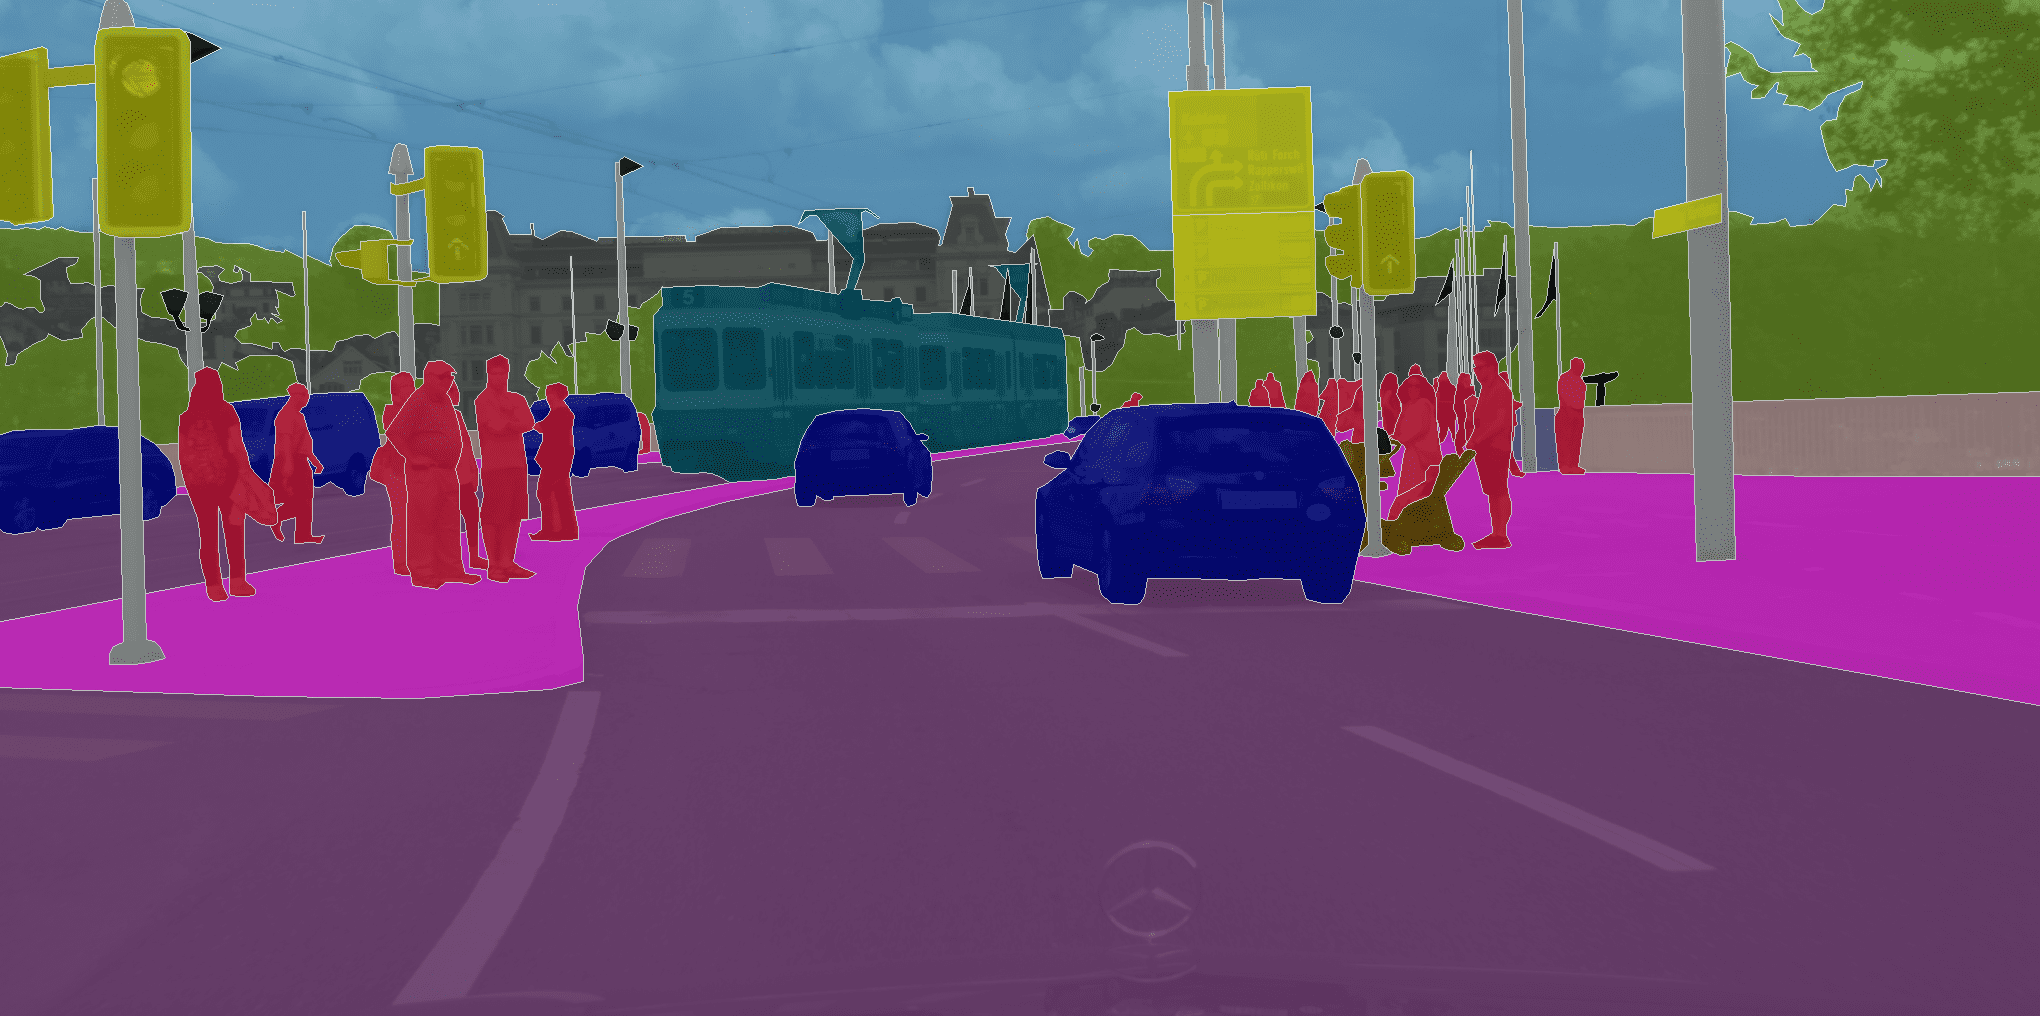
\includegraphics[width=\linewidth, height=0.2\textheight]{Images/Chapter2/Cityscapes/zuerich00.png}
		\caption{برچسب‌گذاری دقیق}
		\label{f64}
	\end{subfigure}\hfil
	\begin{subfigure}{0.45\textwidth}
		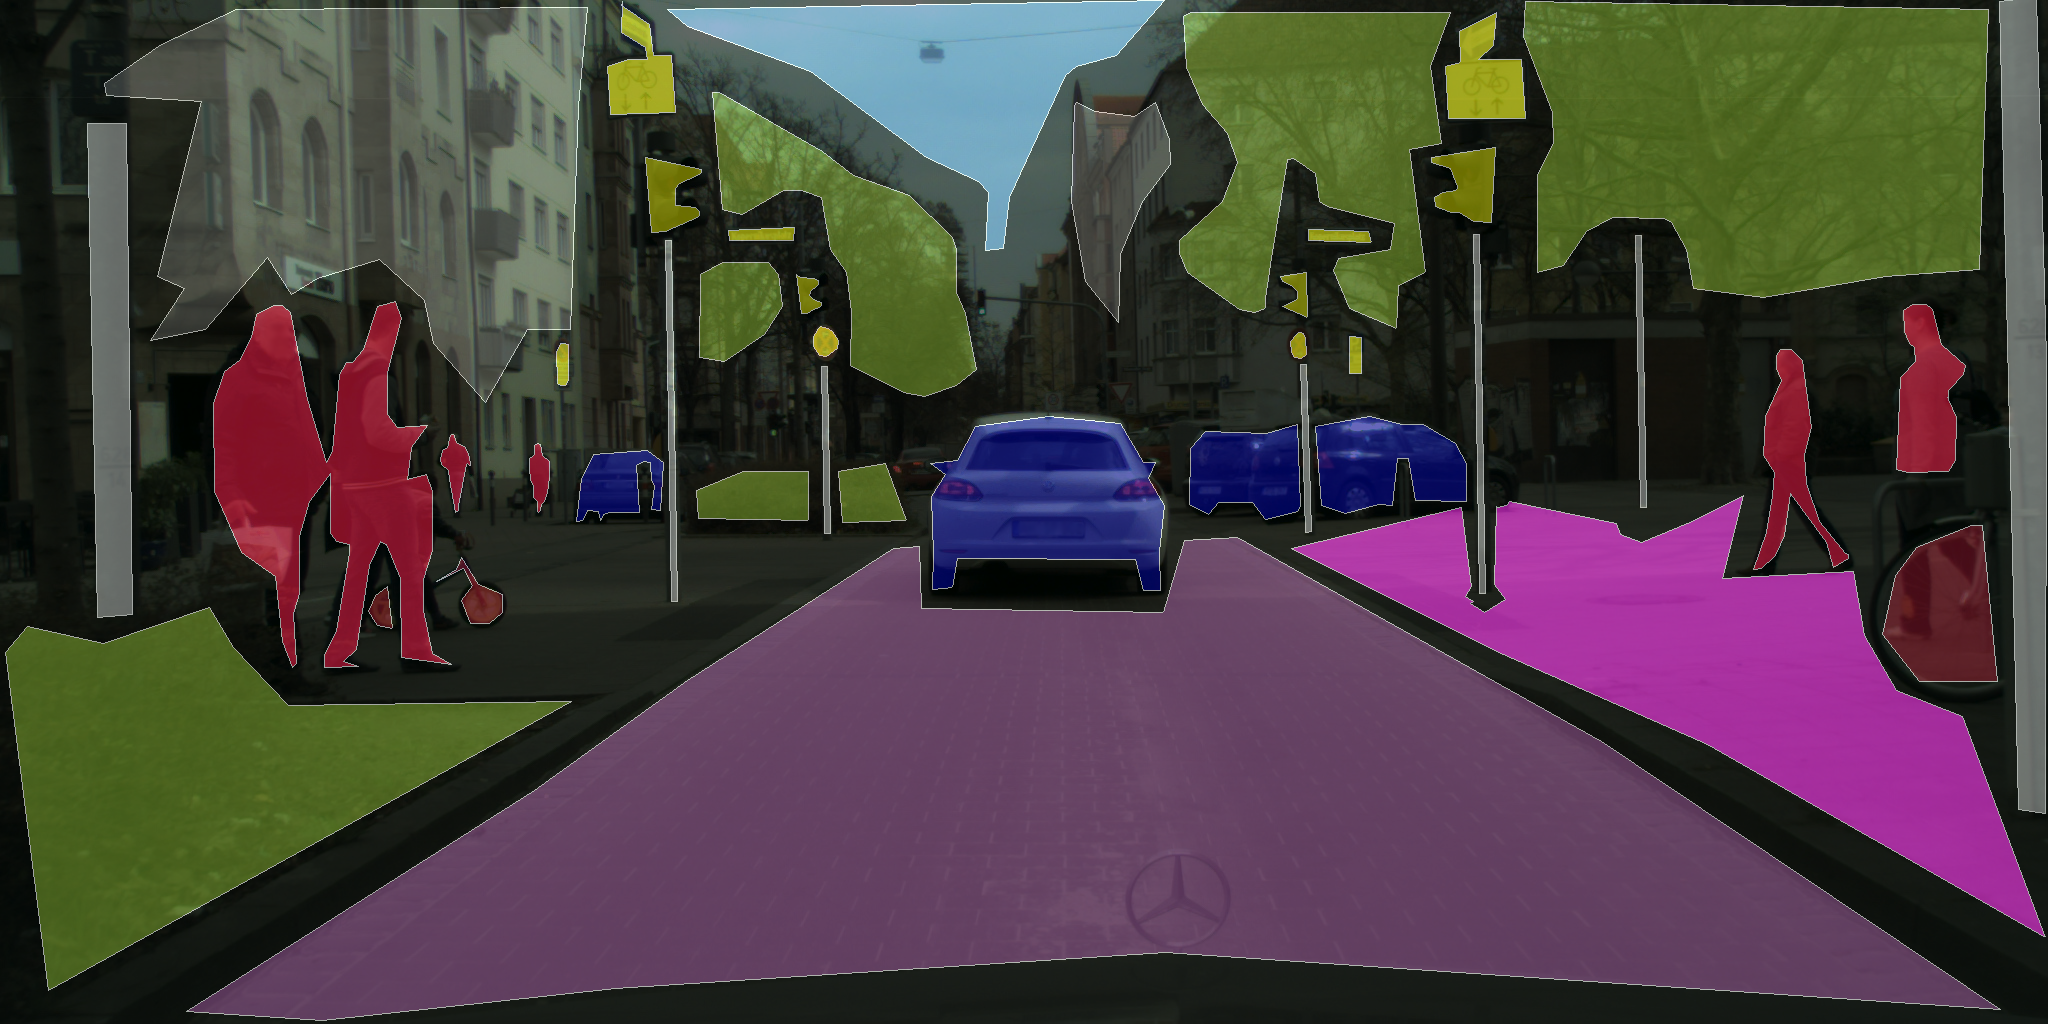
\includegraphics[width=\linewidth, height=0.2\textheight]{Images/Chapter2/Cityscapes/nuremberg00.png}
		\caption{برچسب‌گذاری خشن}
		\label{f65}
	\end{subfigure}
	\caption{انواع بر‌چسب‌گذاری دادگان \lr{Cityscapes}}
	\label{fig:fig1}
\end{figure}

ما در این پژوهش از ۵۰۰۰ تصویر با برچسب‌گذاری شده به شیوه دقیق استفاده خواهیم کرد، چراکه مراجع مورد استفاده قرار گرفته نیز از این نوع برچسب‌گذاری برای مقایسه استفاده کرده اند.

\subsection{مجموعه داده \lr{CamVid}}

در سال ۲۰۰۷، پایگاه داده ویدیویی با برچسب‌گذاری شهری کمبریج (\verb*|CamVid|)، از اولین مجموعه‌های داده تقسیم‌بندی معنایی برای خودروهای خودران، منتشر شد که در آن، ۷۰۰ تصویر از یک دنباله ویدیویی با مدت زمان ۱۰ دقیقه برچسب‌گذاری شد. برای گرفتن ویدیو، دوربین در جلوی ماشین قرار گرفته که دیدگاه مشابهی با راننده دارد. در این مجموعه داده ۳۲ دسته بندی معنایی وجود دارد.

\section{معیار‌های ارزیابی}

\subsubsection{زمان استنتاج}

برای اندازه‌گیری زمان استنتاج از معیار
\verb*|fps|
\LTRfootnote{Frame per second}
استفاده می‌کنیم تا سرعت زمان استنتاج مدل‌ها را با یکدیگر بررسی کنیم. به طبع هر چه
\verb*|fps|
بالاتری داشته باشیم برای ما مطلوب‌تر خواهد بود.


\subsubsection{بهره‌وری منابع}

در این معیار به سه مشخصه زیر می‌پردازیم تا دید بهتری به مقیاس هر مدل پیدا کنیم:

\begin{itemize}
	\item تعداد پارامتر ها: هر چه تعداد نورون‌های بیشتری داشته باشیم مدل سنگین تر می‌شود. تلاش بر آن است که مدل پیشنهادی سبک‌وزن (\lr{lightweight}) باشد.
	\item میزان مصرف مموری: متناسب با پیچیدگی مدل در تعداد و نوع عملیات‌ها میزان مصرف مموری در حین اجرا متغیر است.
	\item میزان مصرف حافظه: این مقدار با تعداد پارامتر‌ها نسبت مستقیم دارد، اما دید شهودی به مقیاس هر مدل می‌دهد.
\end{itemize}

\subsubsection{میانگین اشتراک بر اجتماع}

میانگین اشتراک بر اجتماع
\LTRfootnote{Mean intersection-over-union (Mean IoU)}
یک معیار پرکاربرد در مسائل بینایی ماشین
\LTRfootnote{Computer vision}
است که برای ارزیابی عملکرد مدل‌ها مورد استفاده قرار می‌گیرد و به وسیله محاسبه میزان تطابق بین ماسک تشخیص
\LTRfootnote{Prediction mask}
شیء پیش‌بینی شده توسط مدل و ماسک واقعی در تصویر عمل می‌کند. برای محاسبه این معیار، ابتدا
\verb*|IoU|
یا اشتراک بر اجتماع برای هر شیء در تصویر محاسبه می‌شود، سپس از آن‌ها میانگین گرفته می‌شود تا عملکرد کلی مدل در تشخیص شیء مورد ارزیابی قرار گیرد.

در اینجا اشتراک بر اجتماع هر دسته و میانگین کلی به صورت جدا سنجیده و مقایسه می‌شود.

\section{شرایط آزمایش}

برای ایجاد یک مقایسه عادلانه، دادگان مورد استفاده قرار گرفته را به دو بخش مجموعه‌داده آموزشی
\LTRfootnote{Training set}
و مجموعه‌داده صحبت‌سنجی
\LTRfootnote{Validation set}
تقسیم کردیم. تقسیم‌بندی به همانگونه که در دادگان اولیه انجام‌شده بود نگه‌داشته شد تا در مقایسه با مقاله‌های معتبر دچار مشکل نشویم.
تمامی مدل‌های پیاده سازی شده در چهارچوب پیاده‌سازی پایتورچ
\LTRfootnote{PyTorch framework}
پیاده‌سازی شده اند و تمامی آن‌ها بر روی سخت‌افزای با پردازنده
\verb*|AMD|
\verb*|Ryzen7|
\verb*|3.20|
\verb*|GHz|
و کارت گرافیکی
\verb*|NVIDIA|
\verb*|GeForce|
\verb*|GTX|
\verb*|3060|
\verb*|6GB|
انجام شده است.
\section{نتایج آزمایش و مقایسه}

در ابتدا به بررسی سرعت پردازش (
\verb*|fps|
) پرداخته می‌شود. در آزمایش فرض شده ۱۰ دسته‌بندی اشیاء داشته و تمامی تصاویر دارای ۳ کانال رنگی هستند. به دلیل محدودیت سخت‌افزاری روی پردازنده گرافیکی این مقایسه بر روی تصاویر با ابعاد ۲۰۴۸ در ۱۰۲۴ انجام نشده است. نتایج در جدول زیر قابل مشاهده است.

\begin{table}[ht]
	\centering
	\renewcommand{\arraystretch}{1.5}
	\begin{tabular}{|c|c|c|c|c|}
		\hline
		& $64$ \lr{x} $128$ & $128$ \lr{x} $256$ & $256$ \lr{x} $512$ & $512$ \lr{x} $1024$ \\ \hline
		\lr{UNet} 		& $99.11$ & $95.47$ & $42.8$ & $7.42$ \\ \hline
		\lr{SQNet}  	& $94.01$ & $96.06$ & $41.86$ & $19.66$ \\ \hline
		\lr{ENet}  		& $70.55$ & $64.81$ & $34.98$ & $3.46$ \\ \hline
		\lr{FastSCNN}  	& $46.63$ & $46.55$ & $47.00$ & $33.63$ \\ \hline
		\lr{SegNet} 	& $18.84$ & $17.65$ & $14.99$ & $12.92$ \\ \hline
	\end{tabular}
	\caption{مقایسه شاخص \lr{fps}}
	\label{Table1}
\end{table}

علت گرفتن نتایج ضعیف‌تر نسبت به مقاله‌های اصلی، ضعیف‌تر بودن کارت گرافیکی استفاده شده و تفاوت‌های احتمالی در پیاده‌سازی‌های صورت گرفته است.



\section{خلاصه}
\chapter{نتیجه گیری، جمع ‌بندی و پیشنهادات}

\section{جمع‌بندي و نتيجه‌گيري}

در این پژوهش به بررسی معماری‌های مختلف برای حل مسئله تقسیم‌بندی معنایی تصاویر در حوزه خودرو‌های خودران با استفاده از روش های یادگیری عمیق پرداختیم. همانطور که در مقدمه به طور مفصل‌تر به آن پرداخته شد، مدل‌های مورد استفاده برای این حوزه بخصوص، علاوه بر دقت نیاز به سرعت عمل بالا نیز دارند که معیار مهمی در ارزیابی نهایی آنها است.

در فصل دوم، به مطالعه مفاهیم پرتکرار این حوزه پرداخته و معماری‌های مورد استفاده، نظیر معماری رمزگذار-رمزگشا، را معرفی کردیم که کاربرد گسترده ای در مدل‌های مطرح برای این حوزه دارد و به جزئیات آن پرداختیم. سپس چندین معماری مطرح در حوزه تقسیم‌بندی معنایی را معرفی کردیم که از دقت بالایی برخوردار بوده، اما عملکرد خوبی در پردازش آنی ندارند که مشخصه مهمی در ارزیابی نهایی است.

در فصل سوم، به طور عمیق وارد معماری منحصر به فرد مدل‌های پیشنهادی و اجزای کلیدی آنها شدیم و نقاط ضعف و قوت هر یک را بررسی و مقایسه کردیم. با وجود مدل‌های متعدد در حوزه تقسیم‌بندی معنایی، می‌توان گفت اکثر مدل‌ها از معماری رمزگذار-رمزگشا و یا مشابه آن استفاده می‌کنند تا بتوانند عملکرد بهینه‌تری در سرعت پردازش بدست آورند. متوجه شدیم با تغییر بر روی اجزای این معماری، مانند تعداد لایه ها، نوع توابع‌فعال‌ساز، حذف نرمال‌سازی، و موارد مشابه می‌توان بر تعداد وزن‌های مورد نیاز و میزان محاسبات لازم را کاهش داد و در نهایت بر روی سرعت پردازش تاثیر مثبت گذاشت. همچنین می‌توان با تغییر در معماری مانند افزودن پرش، ترکیب داده‌های لایه‌ها و استفاده از معماری دو-شاخه بر، دقت و کیفیت تصویر بازسازی شده را بهبود داد.

در فصل چهارم، آزمایش‌های و نتایج، به آموزش و ارزیابی معماری‌های مطرح شده پرداختیم. ارزیابی‌های صورت گرفته نه تنها بر روی دقت و شاخص بازسازی تصاویر بود، بلکه بر روی سرعت پردازش و مصرف منابع مدل‌ها نیز تمرکز داشتیم. طی مقایسه عملکرد مدل‌ها متوجه شدیم استفاده از معماری دو-شاخه در معماری اولیه رمزگذار-رمزگشا تاثیر مثبتی بر روی سرعت پردازش می‌گذارد و در عین حال دقت مدل دچار نوسان چندانی نمی‌شود که مطلوب ما است.

\section{پیشنهادات و کار‌های آتی}

روش‌های مورد بحث و بررسی قرار گرفته داخل این پروژه همگی بر روی تصاویر تمرکز داشته‌اند؛ به گونه‌ای که برای پردازش ویدیو، هر فریم به تنهایی و مجزا از فریم‌های پیشین پردازش می‌شود. چالش روش فعلی آن است که امکان تغییر دسته‌بندی ها بین دو تصویر متوالی در یک ویدیو وجود دارد و سازوکاری برای کاهش و یا جلو‌گیری از آن نداریم. مدل‌های نوین‌تر تقسیم‌بندی معنایی ویدیویی
\LTRfootnote{Video semantic segmentation}
نظیر 
\verb*|TMANET|
\cite{wang2021temporal}
\LTRfootnote{Temporal Memory Attention Network}
به حل این مشکل می‌پردازند. در این گونه مدل های، یک یا چند تصویر گذشته بر روی تقسیم‌بندی معنایی تصویر بعدی، به صورت وزن‌دار، تاثیرگذار هستند و بنابراین امکان تغییر ناگهانی یک دسته به دلیل خطای مدل و یا شرایط جدید محیطی کاهش میابد. هرچند استفاده از این گونه مدل‌های ویدیووی در حوزه خودرو‌های خودران مانند مدل‌های تقسیم‌بندی تصویر مرسوم نیست، تمرکز بیشتر بر روی این مدل ها و بهینه‌سازی آنها برای پردازش سریع‌تر پیشنهاد می‌شود.


%--------------------------------------------------------------------------appendix( مراجع و پیوست ها)
\chapterfont{\vspace*{-2em}\centering\LARGE}%

\appendix
\bibliographystyle{unsrt-fa}
\bibliography{references}
%--------------------------------------------------------------------------index(نمایه)
%اگر مایل به داشتن صفحه نمایه نیستید، خط زیر را غیر فعال کنید.
\pagestyle{style7}
\printindex
\pagestyle{style7}
%کلمات کلیدی انگلیسی
\latinkeywords{Artificial intelligence, Self-driving cars, Deep learning, Semantic segmentation, Fast image semantic segmentation}
%چکیده انگلیسی

\en-abstract{
Autonomous vehicles require a precise understanding of their surroundings to make informed decisions and navigate safely in various environments. Semantic segmentation, from its inception, stands as one of the fundamental stages in the process of analyzing images and extracting useful information for decision-making in such systems. It plays a vital role in detecting environmental objects, enabling the accurate identification of various entities including roads, pedestrians, other vehicles, and obstacles. Deep learning methods have significantly improved semantic segmentation, surpassing traditional approaches in performance. This project delves into recent advancements in semantic image segmentation for autonomous vehicles using deep learning methods. We investigate various architectures of deep learning in the context of rapid semantic segmentation, comparing their strengths and weaknesses for the specific task of autonomous driving. Additionally, the datasets used for training and evaluating semantic segmentation models in this domain are scrutinized, employing them to assess different deep learning models. In conclusion, a summary of the examined models is provided, along with suggestions for future research aimed at enhancing the sustainability, efficiency, and general applicability of real-time semantic segmentation systems based on deep learning for autonomous vehicles.
}

\newpage
\thispagestyle{empty}
\begin{latin}
\section*{\LARGE\centering Abstract}

\een-abstract

\vspace*{.5cm}
{\large\textbf{Key Words:}}\par
\vspace*{.5cm}
\elatinkeywords
\end{latin}
\baselineskip=.6cm
\begin{latin}

\latinfaculty{Department of Computer Engineering}


\latintitle{Image Semantic Segmentation for Autonomous Driving with Deep Learning}


\firstlatinsupervisor{Dr. Ehsan Nazerfard}

%\secondlatinsupervisor{Second Supervisor}

%\firstlatinadvisor{Dr. }

%\secondlatinadvisor{Second Advisor}

\latinname{Keivan}

\latinsurname{Ipchi Hagh}

\latinthesisdate{March 2024}

\latinvtitle
\end{latin}

\end{document}